\documentclass[1p]{elsarticle_modified}
%\bibliographystyle{elsarticle-num}

%\usepackage[colorlinks]{hyperref}
%\usepackage{abbrmath_seonhwa} %\Abb, \Ascr, \Acal ,\Abf, \Afrak
\usepackage{amsfonts}
\usepackage{amssymb}
\usepackage{amsmath}
\usepackage{amsthm}
\usepackage{scalefnt}
\usepackage{amsbsy}
\usepackage{kotex}
\usepackage{caption}
\usepackage{subfig}
\usepackage{color}
\usepackage{graphicx}
\usepackage{xcolor} %% white, black, red, green, blue, cyan, magenta, yellow
\usepackage{float}
\usepackage{setspace}
\usepackage{hyperref}

\usepackage{tikz}
\usetikzlibrary{arrows}

\usepackage{multirow}
\usepackage{array} % fixed length table
\usepackage{hhline}

%%%%%%%%%%%%%%%%%%%%%
\makeatletter
\renewcommand*\env@matrix[1][\arraystretch]{%
	\edef\arraystretch{#1}%
	\hskip -\arraycolsep
	\let\@ifnextchar\new@ifnextchar
	\array{*\c@MaxMatrixCols c}}
\makeatother %https://tex.stackexchange.com/questions/14071/how-can-i-increase-the-line-spacing-in-a-matrix
%%%%%%%%%%%%%%%

\usepackage[normalem]{ulem}

\newcommand{\msout}[1]{\ifmmode\text{\sout{\ensuremath{#1}}}\else\sout{#1}\fi}
%SOURCE: \msout is \stkout macro in https://tex.stackexchange.com/questions/20609/strikeout-in-math-mode

\newcommand{\cancel}[1]{
	\ifmmode
	{\color{red}\msout{#1}}
	\else
	{\color{red}\sout{#1}}
	\fi
}

\newcommand{\add}[1]{
	{\color{blue}\uwave{#1}}
}

\newcommand{\replace}[2]{
	\ifmmode
	{\color{red}\msout{#1}}{\color{blue}\uwave{#2}}
	\else
	{\color{red}\sout{#1}}{\color{blue}\uwave{#2}}
	\fi
}

\newcommand{\Sol}{\mathcal{S}} %segment
\newcommand{\D}{D} %diagram
\newcommand{\A}{\mathcal{A}} %arc


%%%%%%%%%%%%%%%%%%%%%%%%%%%%%5 test

\def\sl{\operatorname{\textup{SL}}(2,\Cbb)}
\def\psl{\operatorname{\textup{PSL}}(2,\Cbb)}
\def\quan{\mkern 1mu \triangleright \mkern 1mu}

\theoremstyle{definition}
\newtheorem{thm}{Theorem}[section]
\newtheorem{prop}[thm]{Proposition}
\newtheorem{lem}[thm]{Lemma}
\newtheorem{ques}[thm]{Question}
\newtheorem{cor}[thm]{Corollary}
\newtheorem{defn}[thm]{Definition}
\newtheorem{exam}[thm]{Example}
\newtheorem{rmk}[thm]{Remark}
\newtheorem{alg}[thm]{Algorithm}

\newcommand{\I}{\sqrt{-1}}
\begin{document}

%\begin{frontmatter}
%
%\title{Boundary parabolic representations of knots up to 8 crossings}
%
%%% Group authors per affiliation:
%\author{Yunhi Cho} 
%\address{Department of Mathematics, University of Seoul, Seoul, Korea}
%\ead{yhcho@uos.ac.kr}
%
%
%\author{Seonhwa Kim} %\fnref{s_kim}}
%\address{Center for Geometry and Physics, Institute for Basic Science, Pohang, 37673, Korea}
%\ead{ryeona17@ibs.re.kr}
%
%\author{Hyuk Kim}
%\address{Department of Mathematical Sciences, Seoul National University, Seoul 08826, Korea}
%\ead{hyukkim@snu.ac.kr}
%
%\author{Seokbeom Yoon}
%\address{Department of Mathematical Sciences, Seoul National University, Seoul, 08826,  Korea}
%\ead{sbyoon15@snu.ac.kr}
%
%\begin{abstract}
%We find all boundary parabolic representation of knots up to 8 crossings.
%
%\end{abstract}
%\begin{keyword}
%    \MSC[2010] 57M25 
%\end{keyword}
%
%\end{frontmatter}

%\linenumbers
%\tableofcontents
%
\newcommand\colored[1]{\textcolor{white}{\rule[-0.35ex]{0.8em}{1.4ex}}\kern-0.8em\color{red} #1}%
%\newcommand\colored[1]{\textcolor{white}{ #1}\kern-2.17ex	\textcolor{white}{ #1}\kern-1.81ex	\textcolor{white}{ #1}\kern-2.15ex\color{red}#1	}

{\Large $\underline{12n_{0844}~(K12n_{0844})}$}

\setlength{\tabcolsep}{10pt}
\renewcommand{\arraystretch}{1.6}
\vspace{1cm}\begin{tabular}{m{100pt}>{\centering\arraybackslash}m{274pt}}
\multirow{5}{120pt}{
	\centering
	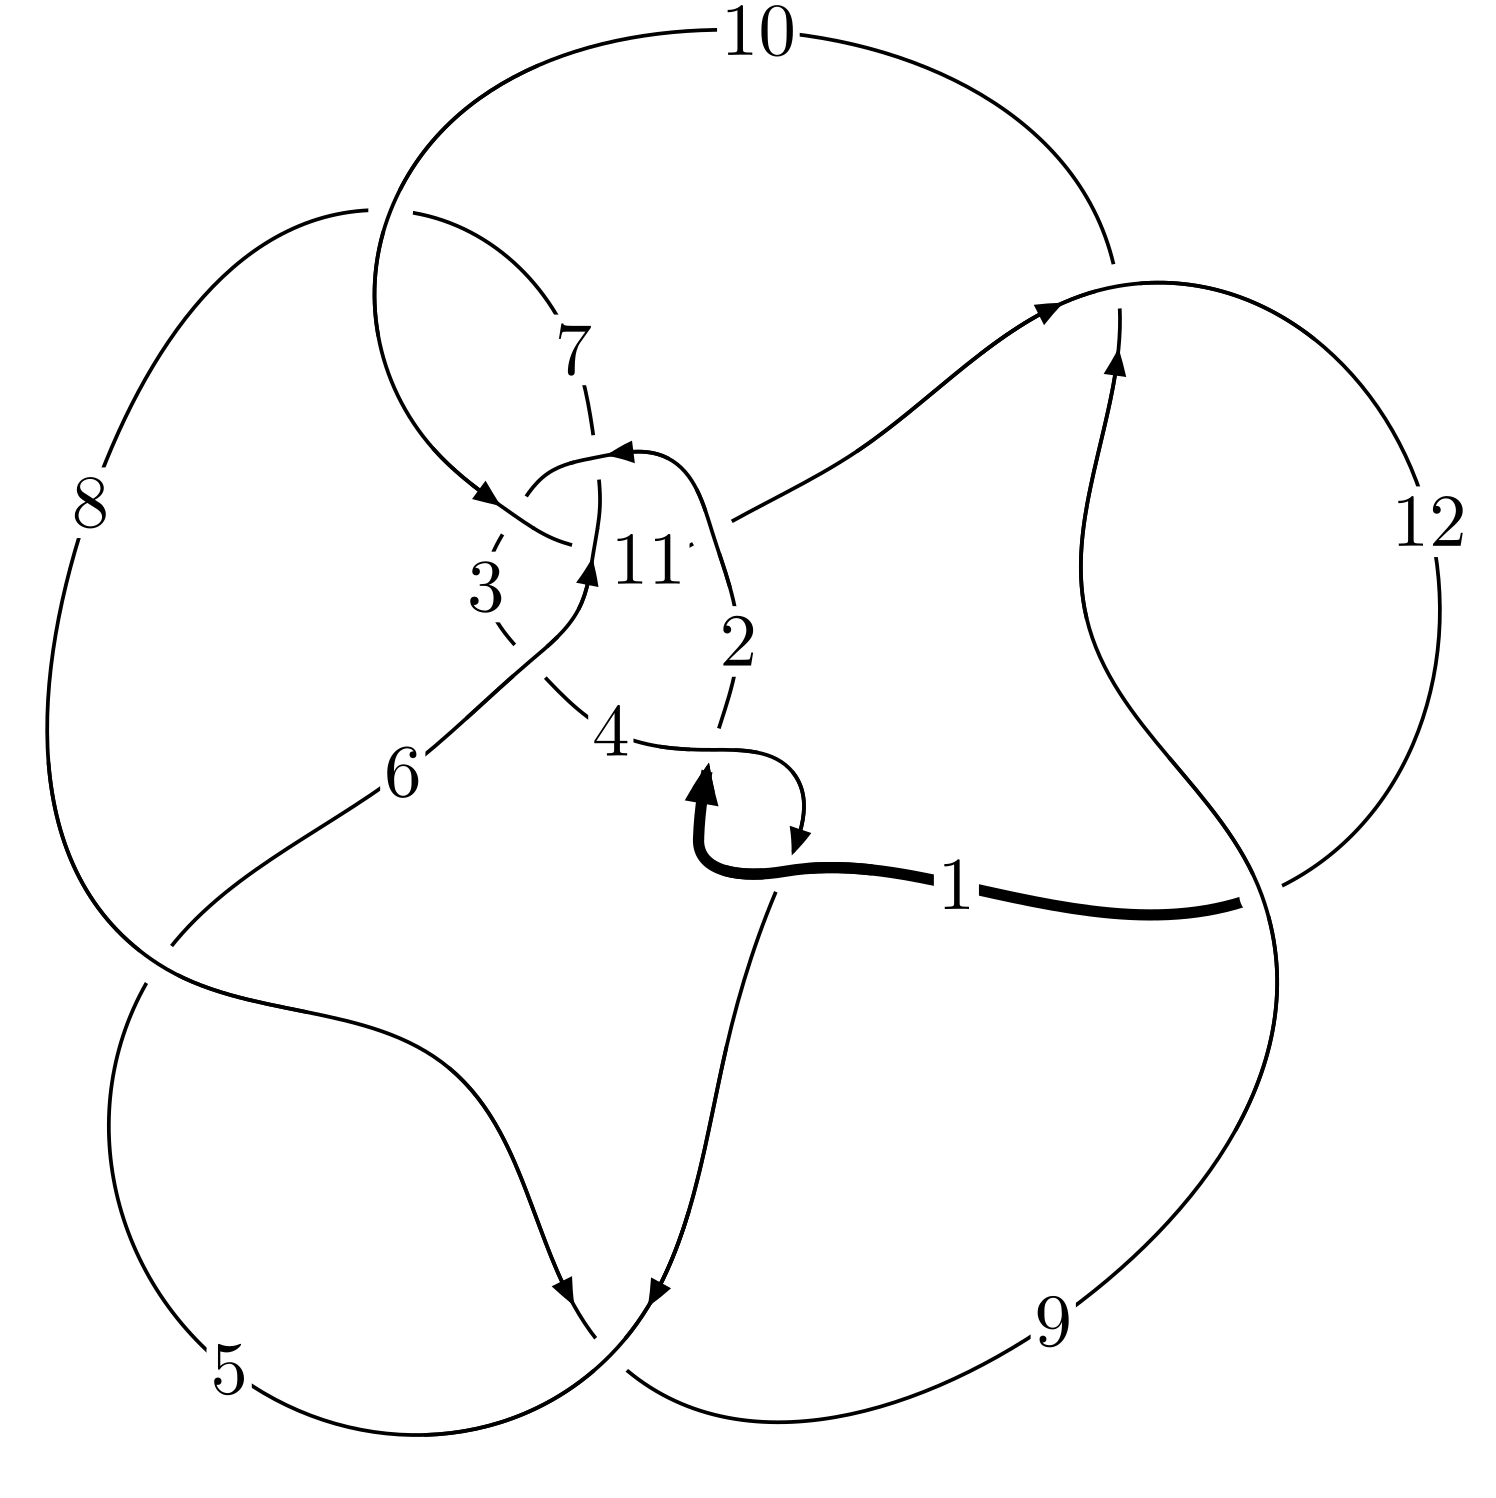
\includegraphics[width=112pt]{../../../GIT/diagram.site/Diagrams/png/2933_12n_0844.png}\\
\ \ \ A knot diagram\footnotemark}&
\allowdisplaybreaks
\textbf{Linearized knot diagam} \\
\cline{2-2}
 &
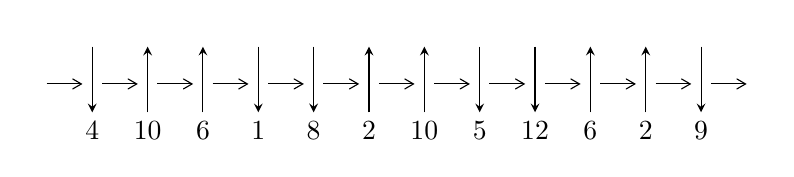
\begin{tikzpicture}[x=20pt, y=17pt]
	% nodes
	\node (C0) at (0, 0) {};
	\node (C1) at (1, 0) {};
	\node (C1U) at (1, +1) {};
	\node (C1D) at (1, -1) {4};

	\node (C2) at (2, 0) {};
	\node (C2U) at (2, +1) {};
	\node (C2D) at (2, -1) {10};

	\node (C3) at (3, 0) {};
	\node (C3U) at (3, +1) {};
	\node (C3D) at (3, -1) {6};

	\node (C4) at (4, 0) {};
	\node (C4U) at (4, +1) {};
	\node (C4D) at (4, -1) {1};

	\node (C5) at (5, 0) {};
	\node (C5U) at (5, +1) {};
	\node (C5D) at (5, -1) {8};

	\node (C6) at (6, 0) {};
	\node (C6U) at (6, +1) {};
	\node (C6D) at (6, -1) {2};

	\node (C7) at (7, 0) {};
	\node (C7U) at (7, +1) {};
	\node (C7D) at (7, -1) {10};

	\node (C8) at (8, 0) {};
	\node (C8U) at (8, +1) {};
	\node (C8D) at (8, -1) {5};

	\node (C9) at (9, 0) {};
	\node (C9U) at (9, +1) {};
	\node (C9D) at (9, -1) {12};

	\node (C10) at (10, 0) {};
	\node (C10U) at (10, +1) {};
	\node (C10D) at (10, -1) {6};

	\node (C11) at (11, 0) {};
	\node (C11U) at (11, +1) {};
	\node (C11D) at (11, -1) {2};

	\node (C12) at (12, 0) {};
	\node (C12U) at (12, +1) {};
	\node (C12D) at (12, -1) {9};
	\node (C13) at (13, 0) {};

	% arrows
	\draw[->,>={angle 60}]
	(C0) edge (C1) (C1) edge (C2) (C2) edge (C3) (C3) edge (C4) (C4) edge (C5) (C5) edge (C6) (C6) edge (C7) (C7) edge (C8) (C8) edge (C9) (C9) edge (C10) (C10) edge (C11) (C11) edge (C12) (C12) edge (C13) ;	\draw[->,>=stealth]
	(C1U) edge (C1D) (C2D) edge (C2U) (C3D) edge (C3U) (C4U) edge (C4D) (C5U) edge (C5D) (C6D) edge (C6U) (C7D) edge (C7U) (C8U) edge (C8D) (C9U) edge (C9D) (C10D) edge (C10U) (C11D) edge (C11U) (C12U) edge (C12D) ;
	\end{tikzpicture} \\
\hhline{~~} \\& 
\textbf{Solving Sequence} \\ \cline{2-2} 
 &
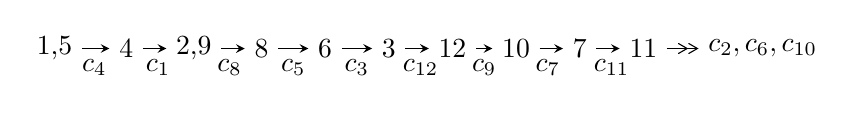
\begin{tikzpicture}[x=23pt, y=7pt]
	% node
	\node (A0) at (-1/8, 0) {1,5};
	\node (A1) at (1, 0) {4};
	\node (A2) at (33/16, 0) {2,9};
	\node (A3) at (25/8, 0) {8};
	\node (A4) at (33/8, 0) {6};
	\node (A5) at (41/8, 0) {3};
	\node (A6) at (49/8, 0) {12};
	\node (A7) at (57/8, 0) {10};
	\node (A8) at (65/8, 0) {7};
	\node (A9) at (73/8, 0) {11};
	\node (C1) at (1/2, -1) {$c_{4}$};
	\node (C2) at (3/2, -1) {$c_{1}$};
	\node (C3) at (21/8, -1) {$c_{8}$};
	\node (C4) at (29/8, -1) {$c_{5}$};
	\node (C5) at (37/8, -1) {$c_{3}$};
	\node (C6) at (45/8, -1) {$c_{12}$};
	\node (C7) at (53/8, -1) {$c_{9}$};
	\node (C8) at (61/8, -1) {$c_{7}$};
	\node (C9) at (69/8, -1) {$c_{11}$};
	\node (A10) at (11, 0) {$c_{2},c_{6},c_{10}$};

	% edge
	\draw[->,>=stealth]	
	(A0) edge (A1) (A1) edge (A2) (A2) edge (A3) (A3) edge (A4) (A4) edge (A5) (A5) edge (A6) (A6) edge (A7) (A7) edge (A8) (A8) edge (A9) ;
	\draw[->>,>={angle 60}]	
	(A9) edge (A10);
\end{tikzpicture} \\ 

\end{tabular} \\

\footnotetext{
The image of knot diagram is generated by the software ``\textbf{Draw programme}" developed by Andrew Bartholomew(\url{http://www.layer8.co.uk/maths/draw/index.htm\#Running-draw}), where we modified some parts for our purpose(\url{https://github.com/CATsTAILs/LinksPainter}).
}\phantom \\ \newline 
\centering \textbf{Ideals for irreducible components\footnotemark of $X_{\text{par}}$} 
 
\begin{align*}
I^u_{1}&=\langle 
b+u,\;a-1,\;u^7-2 u^6+6 u^5-6 u^4+7 u^3-3 u^2-1\rangle \\
I^u_{2}&=\langle 
b+u,\;a+1,\;u^6+u^5+3 u^4+u^3+2 u^2+u+1\rangle \\
I^u_{3}&=\langle 
b+u,\;2 u^{13}+u^{12}+14 u^{11}+u^{10}+36 u^9-14 u^8+40 u^7-42 u^6+19 u^5-39 u^4+11 u^3-8 u^2+2 a+9 u+1,\\
\phantom{I^u_{3}}&\phantom{= \langle  }u^{14}+u^{13}+8 u^{12}+5 u^{11}+23 u^{10}+6 u^9+26 u^8-7 u^7+4 u^6-17 u^5-6 u^4-4 u^3+4 u^2+4 u+1\rangle \\
I^u_{4}&=\langle 
u^{13}+2 u^{12}+9 u^{11}+10 u^{10}+26 u^9+12 u^8+28 u^7-11 u^6+5 u^5-23 u^4- u^2+2 b+7 u+2,\;a-1,\\
\phantom{I^u_{4}}&\phantom{= \langle  }u^{14}+u^{13}+8 u^{12}+5 u^{11}+23 u^{10}+6 u^9+26 u^8-7 u^7+4 u^6-17 u^5-6 u^4-4 u^3+4 u^2+4 u+1\rangle \\
I^u_{5}&=\langle 
-27 u^{13}+169 u^{12}+\cdots+6 b+152,\;38 u^{13}-239 u^{12}+\cdots+6 a-200,\;u^{14}-7 u^{13}+\cdots-16 u+4\rangle \\
I^u_{6}&=\langle 
b+u,\;u^5+3 u^3+a+3 u,\;u^6+3 u^4+u^3+3 u^2+2 u+1\rangle \\
I^u_{7}&=\langle 
- u^3+b-2 u-1,\;a+1,\;u^6+3 u^4+u^3+3 u^2+2 u+1\rangle \\
I^u_{8}&=\langle 
- u^5- u^4-4 u^3-6 u^2+4 b-7 u-6,\;3 u^5+7 u^4+16 u^3+22 u^2+8 a+21 u+10,\\
\phantom{I^u_{8}}&\phantom{= \langle  }u^6+3 u^5+6 u^4+10 u^3+11 u^2+8 u+4\rangle \\
I^u_{9}&=\langle 
u^5+u^3-2 a u+2 u^2+2 b-3 u+1,\\
\phantom{I^u_{9}}&\phantom{= \langle  }u^5 a+25 u^5+3 u^3 a+20 u^4+4 u^2 a+71 u^3+2 a^2+a u+112 u^2+9 a+53 u+141,\\
\phantom{I^u_{9}}&\phantom{= \langle  }u^6+u^5+3 u^4+5 u^3+3 u^2+6 u+1\rangle \\
\\
\end{align*}
\raggedright * 9 irreducible components of $\dim_{\mathbb{C}}=0$, with total 85 representations.\\
\footnotetext{All coefficients of polynomials are rational numbers. But the coefficients are sometimes approximated in decimal forms when there is not enough margin.}
\newpage
\renewcommand{\arraystretch}{1}
\centering \section*{I. $I^u_{1}= \langle b+u,\;a-1,\;u^7-2 u^6+6 u^5-6 u^4+7 u^3-3 u^2-1 \rangle$}
\flushleft \textbf{(i) Arc colorings}\\
\begin{tabular}{m{7pt} m{180pt} m{7pt} m{180pt} }
\flushright $a_{1}=$&$\begin{pmatrix}0\\u\end{pmatrix}$ \\
\flushright $a_{5}=$&$\begin{pmatrix}1\\0\end{pmatrix}$ \\
\flushright $a_{4}=$&$\begin{pmatrix}1\\- u^2\end{pmatrix}$ \\
\flushright $a_{2}=$&$\begin{pmatrix}- u\\u^3+u\end{pmatrix}$ \\
\flushright $a_{9}=$&$\begin{pmatrix}1\\- u\end{pmatrix}$ \\
\flushright $a_{8}=$&$\begin{pmatrix}- u+1\\- u\end{pmatrix}$ \\
\flushright $a_{6}=$&$\begin{pmatrix}u^2- u+1\\u^2\end{pmatrix}$ \\
\flushright $a_{3}=$&$\begin{pmatrix}u^6-2 u^5+4 u^4-3 u^3+2 u^2+1\\u^6- u^5+2 u^4- u^2\end{pmatrix}$ \\
\flushright $a_{12}=$&$\begin{pmatrix}u\\- u^2+u\end{pmatrix}$ \\
\flushright $a_{10}=$&$\begin{pmatrix}u^2+1\\- u^3+u^2- u\end{pmatrix}$ \\
\flushright $a_{7}=$&$\begin{pmatrix}u^6- u^5+3 u^4- u^3+2 u^2- u+1\\2 u^5-3 u^4+5 u^3-3 u^2- u-1\end{pmatrix}$ \\
\flushright $a_{11}=$&$\begin{pmatrix}- u^5+u^4-2 u^3+u\\u^6-3 u^5+5 u^4-5 u^3+2 u^2+u+1\end{pmatrix}$\\&\end{tabular}
\flushleft \textbf{(ii) Obstruction class $= -1$}\\~\\
\flushleft \textbf{(iii) Cusp Shapes $= 3 u^6-6 u^5+15 u^4-18 u^3+15 u^2-12 u+3$}\\~\\
\newpage\renewcommand{\arraystretch}{1}
\flushleft \textbf{(iv) u-Polynomials at the component}\newline \\
\begin{tabular}{m{50pt}|m{274pt}}
Crossings & \hspace{64pt}u-Polynomials at each crossing \\
\hline $$\begin{aligned}c_{1},c_{4},c_{5}\\c_{8},c_{9},c_{12}\end{aligned}$$&$\begin{aligned}
&u^7-2 u^6+6 u^5-6 u^4+7 u^3-3 u^2-1
\end{aligned}$\\
\hline $$\begin{aligned}c_{2},c_{6},c_{10}\end{aligned}$$&$\begin{aligned}
&u^7-5 u^6+7 u^5-3 u^3-2 u^2+u-1
\end{aligned}$\\
\hline $$\begin{aligned}c_{3},c_{7},c_{11}\end{aligned}$$&$\begin{aligned}
&u^7+6 u^6+15 u^5+17 u^4+7 u^3-3 u^2-2 u+2
\end{aligned}$\\
\hline
\end{tabular}\\~\\
\newpage\renewcommand{\arraystretch}{1}
\flushleft \textbf{(v) Riley Polynomials at the component}\newline \\
\begin{tabular}{m{50pt}|m{274pt}}
Crossings & \hspace{64pt}Riley Polynomials at each crossing \\
\hline $$\begin{aligned}c_{1},c_{4},c_{5}\\c_{8},c_{9},c_{12}\end{aligned}$$&$\begin{aligned}
&y^7+8 y^6+26 y^5+36 y^4+9 y^3-21 y^2-6 y-1
\end{aligned}$\\
\hline $$\begin{aligned}c_{2},c_{6},c_{10}\end{aligned}$$&$\begin{aligned}
&y^7-11 y^6+43 y^5-60 y^4+13 y^3-10 y^2-3 y-1
\end{aligned}$\\
\hline $$\begin{aligned}c_{3},c_{7},c_{11}\end{aligned}$$&$\begin{aligned}
&y^7-6 y^6+35 y^5-47 y^4+67 y^3-105 y^2+16 y-4
\end{aligned}$\\
\hline
\end{tabular}\\~\\
\newpage\flushleft \textbf{(vi) Complex Volumes and Cusp Shapes}
$$\begin{array}{c|c|c}  
\text{Solutions to }I^u_{1}& \I (\text{vol} + \sqrt{-1}CS) & \text{Cusp shape}\\
 \hline 
\begin{aligned}
u &= \phantom{-}0.820643\phantom{ +0.000000I} \\
a &= \phantom{-}1.00000\phantom{ +0.000000I} \\
b &= -0.820643\phantom{ +0.000000I}\end{aligned}
 & \phantom{-}4.61500\phantom{ +0.000000I} & -1.20760\phantom{ +0.000000I} \\ \hline\begin{aligned}
u &= \phantom{-}0.29696 + 1.40213 I \\
a &= \phantom{-}1.00000\phantom{ +0.000000I} \\
b &= -0.29696 - 1.40213 I\end{aligned}
 & \phantom{-}9.73442 - 0.66586 I & \phantom{-}5.31181 - 1.86830 I \\ \hline\begin{aligned}
u &= \phantom{-}0.29696 - 1.40213 I \\
a &= \phantom{-}1.00000\phantom{ +0.000000I} \\
b &= -0.29696 + 1.40213 I\end{aligned}
 & \phantom{-}9.73442 + 0.66586 I & \phantom{-}5.31181 + 1.86830 I \\ \hline\begin{aligned}
u &= -0.196466 + 0.415967 I \\
a &= \phantom{-}1.00000\phantom{ +0.000000I} \\
b &= \phantom{-}0.196466 - 0.415967 I\end{aligned}
 & \phantom{-}0.207126 + 1.131650 I & \phantom{-}1.63683 - 6.29574 I \\ \hline\begin{aligned}
u &= -0.196466 - 0.415967 I \\
a &= \phantom{-}1.00000\phantom{ +0.000000I} \\
b &= \phantom{-}0.196466 + 0.415967 I\end{aligned}
 & \phantom{-}0.207126 - 1.131650 I & \phantom{-}1.63683 + 6.29574 I \\ \hline\begin{aligned}
u &= \phantom{-}0.48918 + 1.60119 I \\
a &= \phantom{-}1.00000\phantom{ +0.000000I} \\
b &= -0.48918 - 1.60119 I\end{aligned}
 & -19.6512 - 14.5525 I & \phantom{-}7.15517 + 5.93239 I \\ \hline\begin{aligned}
u &= \phantom{-}0.48918 - 1.60119 I \\
a &= \phantom{-}1.00000\phantom{ +0.000000I} \\
b &= -0.48918 + 1.60119 I\end{aligned}
 & -19.6512 + 14.5525 I & \phantom{-}7.15517 - 5.93239 I\\
 \hline 
 \end{array}$$\newpage\newpage\renewcommand{\arraystretch}{1}
\centering \section*{II. $I^u_{2}= \langle b+u,\;a+1,\;u^6+u^5+3 u^4+u^3+2 u^2+u+1 \rangle$}
\flushleft \textbf{(i) Arc colorings}\\
\begin{tabular}{m{7pt} m{180pt} m{7pt} m{180pt} }
\flushright $a_{1}=$&$\begin{pmatrix}0\\u\end{pmatrix}$ \\
\flushright $a_{5}=$&$\begin{pmatrix}1\\0\end{pmatrix}$ \\
\flushright $a_{4}=$&$\begin{pmatrix}1\\- u^2\end{pmatrix}$ \\
\flushright $a_{2}=$&$\begin{pmatrix}- u\\u^3+u\end{pmatrix}$ \\
\flushright $a_{9}=$&$\begin{pmatrix}-1\\- u\end{pmatrix}$ \\
\flushright $a_{8}=$&$\begin{pmatrix}- u-1\\- u\end{pmatrix}$ \\
\flushright $a_{6}=$&$\begin{pmatrix}u^2+u+1\\u^2\end{pmatrix}$ \\
\flushright $a_{3}=$&$\begin{pmatrix}u^5+u^4+2 u^3- u\\- u^4- u^3-3 u^2- u-1\end{pmatrix}$ \\
\flushright $a_{12}=$&$\begin{pmatrix}u\\u^2+u\end{pmatrix}$ \\
\flushright $a_{10}=$&$\begin{pmatrix}- u^2-1\\- u^3- u^2- u\end{pmatrix}$ \\
\flushright $a_{7}=$&$\begin{pmatrix}0\\u^4+u^3+3 u^2+u+1\end{pmatrix}$ \\
\flushright $a_{11}=$&$\begin{pmatrix}- u^5- u^4-2 u^3+u\\0\end{pmatrix}$\\&\end{tabular}
\flushleft \textbf{(ii) Obstruction class $= 1$}\\~\\
\flushleft \textbf{(iii) Cusp Shapes $= -9 u^5-6 u^4-21 u^3+3 u^2-9 u$}\\~\\
\newpage\renewcommand{\arraystretch}{1}
\flushleft \textbf{(iv) u-Polynomials at the component}\newline \\
\begin{tabular}{m{50pt}|m{274pt}}
Crossings & \hspace{64pt}u-Polynomials at each crossing \\
\hline $$\begin{aligned}c_{1},c_{5},c_{9}\end{aligned}$$&$\begin{aligned}
&u^6- u^5+3 u^4- u^3+2 u^2- u+1
\end{aligned}$\\
\hline $$\begin{aligned}c_{2},c_{6},c_{10}\end{aligned}$$&$\begin{aligned}
&u^6+4 u^5+5 u^4+3 u^3+2 u^2+1
\end{aligned}$\\
\hline $$\begin{aligned}c_{3},c_{7},c_{11}\end{aligned}$$&$\begin{aligned}
&u^6+2 u^5- u^4-3 u^3+u^2- u+2
\end{aligned}$\\
\hline $$\begin{aligned}c_{4},c_{8},c_{12}\end{aligned}$$&$\begin{aligned}
&u^6+u^5+3 u^4+u^3+2 u^2+u+1
\end{aligned}$\\
\hline
\end{tabular}\\~\\
\newpage\renewcommand{\arraystretch}{1}
\flushleft \textbf{(v) Riley Polynomials at the component}\newline \\
\begin{tabular}{m{50pt}|m{274pt}}
Crossings & \hspace{64pt}Riley Polynomials at each crossing \\
\hline $$\begin{aligned}c_{1},c_{4},c_{5}\\c_{8},c_{9},c_{12}\end{aligned}$$&$\begin{aligned}
&y^6+5 y^5+11 y^4+11 y^3+8 y^2+3 y+1
\end{aligned}$\\
\hline $$\begin{aligned}c_{2},c_{6},c_{10}\end{aligned}$$&$\begin{aligned}
&y^6-6 y^5+5 y^4+13 y^3+14 y^2+4 y+1
\end{aligned}$\\
\hline $$\begin{aligned}c_{3},c_{7},c_{11}\end{aligned}$$&$\begin{aligned}
&y^6-6 y^5+15 y^4-3 y^3-9 y^2+3 y+4
\end{aligned}$\\
\hline
\end{tabular}\\~\\
\newpage\flushleft \textbf{(vi) Complex Volumes and Cusp Shapes}
$$\begin{array}{c|c|c}  
\text{Solutions to }I^u_{2}& \I (\text{vol} + \sqrt{-1}CS) & \text{Cusp shape}\\
 \hline 
\begin{aligned}
u &= \phantom{-}0.411715 + 0.779640 I \\
a &= -1.00000\phantom{ +0.000000I} \\
b &= -0.411715 - 0.779640 I\end{aligned}
 & \phantom{-}10.29080 - 4.97121 I & \phantom{-}7.46638 + 3.54102 I \\ \hline\begin{aligned}
u &= \phantom{-}0.411715 - 0.779640 I \\
a &= -1.00000\phantom{ +0.000000I} \\
b &= -0.411715 + 0.779640 I\end{aligned}
 & \phantom{-}10.29080 + 4.97121 I & \phantom{-}7.46638 - 3.54102 I \\ \hline\begin{aligned}
u &= -0.459082 + 0.581397 I \\
a &= -1.00000\phantom{ +0.000000I} \\
b &= \phantom{-}0.459082 - 0.581397 I\end{aligned}
 & -0.53119 + 2.71432 I & -2.78148 - 9.27411 I \\ \hline\begin{aligned}
u &= -0.459082 - 0.581397 I \\
a &= -1.00000\phantom{ +0.000000I} \\
b &= \phantom{-}0.459082 + 0.581397 I\end{aligned}
 & -0.53119 - 2.71432 I & -2.78148 + 9.27411 I \\ \hline\begin{aligned}
u &= -0.45263 + 1.46263 I \\
a &= -1.00000\phantom{ +0.000000I} \\
b &= \phantom{-}0.45263 - 1.46263 I\end{aligned}
 & \phantom{-}8.33462 + 8.14586 I & \phantom{-}2.81510 - 6.35297 I \\ \hline\begin{aligned}
u &= -0.45263 - 1.46263 I \\
a &= -1.00000\phantom{ +0.000000I} \\
b &= \phantom{-}0.45263 + 1.46263 I\end{aligned}
 & \phantom{-}8.33462 - 8.14586 I & \phantom{-}2.81510 + 6.35297 I\\
 \hline 
 \end{array}$$\newpage\newpage\renewcommand{\arraystretch}{1}
\centering \section*{III. $I^u_{3}= \langle b+u,\;2 u^{13}+u^{12}+\cdots+2 a+1,\;u^{14}+u^{13}+\cdots+4 u+1 \rangle$}
\flushleft \textbf{(i) Arc colorings}\\
\begin{tabular}{m{7pt} m{180pt} m{7pt} m{180pt} }
\flushright $a_{1}=$&$\begin{pmatrix}0\\u\end{pmatrix}$ \\
\flushright $a_{5}=$&$\begin{pmatrix}1\\0\end{pmatrix}$ \\
\flushright $a_{4}=$&$\begin{pmatrix}1\\- u^2\end{pmatrix}$ \\
\flushright $a_{2}=$&$\begin{pmatrix}- u\\u^3+u\end{pmatrix}$ \\
\flushright $a_{9}=$&$\begin{pmatrix}- u^{13}-\frac{1}{2} u^{12}+\cdots-\frac{9}{2} u-\frac{1}{2}\\- u\end{pmatrix}$ \\
\flushright $a_{8}=$&$\begin{pmatrix}- u^{13}-\frac{1}{2} u^{12}+\cdots-\frac{11}{2} u-\frac{1}{2}\\- u\end{pmatrix}$ \\
\flushright $a_{6}=$&$\begin{pmatrix}-\frac{1}{2} u^{13}- u^{12}+\cdots+\frac{3}{2} u^2-\frac{7}{2} u\\u^2\end{pmatrix}$ \\
\flushright $a_{3}=$&$\begin{pmatrix}\frac{1}{2} u^{13}-4 u^{12}+\cdots-\frac{19}{2} u-2\\-\frac{1}{2} u^{13}-\frac{7}{2} u^{12}+\cdots-6 u-\frac{3}{2}\end{pmatrix}$ \\
\flushright $a_{12}=$&$\begin{pmatrix}\frac{1}{2} u^{13}-\frac{1}{2} u^{12}+\cdots+2 u+\frac{5}{2}\\-\frac{1}{2} u^{13}-\frac{1}{2} u^{12}+\cdots+2 u+\frac{1}{2}\end{pmatrix}$ \\
\flushright $a_{10}=$&$\begin{pmatrix}-\frac{1}{2} u^{13}-\frac{5}{2} u^{12}+\cdots-8 u-\frac{5}{2}\\- u^{13}-\frac{5}{2} u^{12}+\cdots-\frac{11}{2} u-\frac{3}{2}\end{pmatrix}$ \\
\flushright $a_{7}=$&$\begin{pmatrix}- u^{13}-3 u^{12}+\cdots-7 u-1\\-\frac{1}{2} u^{13}-\frac{3}{2} u^{12}+\cdots-3 u-\frac{1}{2}\end{pmatrix}$ \\
\flushright $a_{11}=$&$\begin{pmatrix}\frac{1}{2} u^{13}+u^{12}+\cdots+\frac{11}{2} u+3\\\frac{3}{2} u^{12}+2 u^{11}+\cdots+\frac{9}{2} u+\frac{3}{2}\end{pmatrix}$\\&\end{tabular}
\flushleft \textbf{(ii) Obstruction class $= -1$}\\~\\
\flushleft \textbf{(iii) Cusp Shapes $= -3 u^{13}-4 u^{12}-27 u^{11}-21 u^{10}-83 u^9-23 u^8-97 u^7+43 u^6-14 u^5+86 u^4+16 u^3+12 u^2-29 u-10$}\\~\\
\newpage\renewcommand{\arraystretch}{1}
\flushleft \textbf{(iv) u-Polynomials at the component}\newline \\
\begin{tabular}{m{50pt}|m{274pt}}
Crossings & \hspace{64pt}u-Polynomials at each crossing \\
\hline $$\begin{aligned}c_{1},c_{4},c_{5}\\c_{8}\end{aligned}$$&$\begin{aligned}
&u^{14}+u^{13}+\cdots+4 u+1
\end{aligned}$\\
\hline $$\begin{aligned}c_{2},c_{10}\end{aligned}$$&$\begin{aligned}
&u^{14}+4 u^{13}+\cdots-3 u^2+1
\end{aligned}$\\
\hline $$\begin{aligned}c_{3}\end{aligned}$$&$\begin{aligned}
&u^{14}+14 u^{13}+\cdots+384 u+64
\end{aligned}$\\
\hline $$\begin{aligned}c_{6}\end{aligned}$$&$\begin{aligned}
&u^{14}-8 u^{13}+\cdots-100 u+52
\end{aligned}$\\
\hline $$\begin{aligned}c_{7},c_{11}\end{aligned}$$&$\begin{aligned}
&u^{14}-4 u^{13}+\cdots-27 u+7
\end{aligned}$\\
\hline $$\begin{aligned}c_{9},c_{12}\end{aligned}$$&$\begin{aligned}
&u^{14}-7 u^{13}+\cdots-16 u+4
\end{aligned}$\\
\hline
\end{tabular}\\~\\
\newpage\renewcommand{\arraystretch}{1}
\flushleft \textbf{(v) Riley Polynomials at the component}\newline \\
\begin{tabular}{m{50pt}|m{274pt}}
Crossings & \hspace{64pt}Riley Polynomials at each crossing \\
\hline $$\begin{aligned}c_{1},c_{4},c_{5}\\c_{8}\end{aligned}$$&$\begin{aligned}
&y^{14}+15 y^{13}+\cdots-8 y+1
\end{aligned}$\\
\hline $$\begin{aligned}c_{2},c_{10}\end{aligned}$$&$\begin{aligned}
&y^{14}-22 y^{13}+\cdots-6 y+1
\end{aligned}$\\
\hline $$\begin{aligned}c_{3}\end{aligned}$$&$\begin{aligned}
&y^{14}-2 y^{13}+\cdots+53248 y+4096
\end{aligned}$\\
\hline $$\begin{aligned}c_{6}\end{aligned}$$&$\begin{aligned}
&y^{14}-14 y^{13}+\cdots+6016 y+2704
\end{aligned}$\\
\hline $$\begin{aligned}c_{7},c_{11}\end{aligned}$$&$\begin{aligned}
&y^{14}-16 y^{13}+\cdots+69 y+49
\end{aligned}$\\
\hline $$\begin{aligned}c_{9},c_{12}\end{aligned}$$&$\begin{aligned}
&y^{14}+7 y^{13}+\cdots+80 y+16
\end{aligned}$\\
\hline
\end{tabular}\\~\\
\newpage\flushleft \textbf{(vi) Complex Volumes and Cusp Shapes}
$$\begin{array}{c|c|c}  
\text{Solutions to }I^u_{3}& \I (\text{vol} + \sqrt{-1}CS) & \text{Cusp shape}\\
 \hline 
\begin{aligned}
u &= -0.439663 + 0.679978 I \\
a &= -0.517883 + 0.552774 I \\
b &= \phantom{-}0.439663 - 0.679978 I\end{aligned}
 & \phantom{-}0.33027 + 1.75564 I & \phantom{-}4.64860 - 3.95549 I \\ \hline\begin{aligned}
u &= -0.439663 - 0.679978 I \\
a &= -0.517883 - 0.552774 I \\
b &= \phantom{-}0.439663 + 0.679978 I\end{aligned}
 & \phantom{-}0.33027 - 1.75564 I & \phantom{-}4.64860 + 3.95549 I \\ \hline\begin{aligned}
u &= \phantom{-}0.736420 + 0.153256 I \\
a &= \phantom{-}0.89088 + 1.45567 I \\
b &= -0.736420 - 0.153256 I\end{aligned}
 & \phantom{-}8.26670 - 4.44391 I & \phantom{-}1.65913 + 3.08844 I \\ \hline\begin{aligned}
u &= \phantom{-}0.736420 - 0.153256 I \\
a &= \phantom{-}0.89088 - 1.45567 I \\
b &= -0.736420 + 0.153256 I\end{aligned}
 & \phantom{-}8.26670 + 4.44391 I & \phantom{-}1.65913 - 3.08844 I \\ \hline\begin{aligned}
u &= -0.149559 + 1.356980 I \\
a &= -0.079573 - 0.538803 I \\
b &= \phantom{-}0.149559 - 1.356980 I\end{aligned}
 & \phantom{-}5.20834 + 3.21642 I & \phantom{-}7.19365 - 4.36535 I \\ \hline\begin{aligned}
u &= -0.149559 - 1.356980 I \\
a &= -0.079573 + 0.538803 I \\
b &= \phantom{-}0.149559 + 1.356980 I\end{aligned}
 & \phantom{-}5.20834 - 3.21642 I & \phantom{-}7.19365 + 4.36535 I \\ \hline\begin{aligned}
u &= -0.074998 + 1.387310 I \\
a &= -1.229600 - 0.602077 I \\
b &= \phantom{-}0.074998 - 1.387310 I\end{aligned}
 & \phantom{-}16.9219 + 0.9403 I & \phantom{-}9.61641 - 0.21990 I \\ \hline\begin{aligned}
u &= -0.074998 - 1.387310 I \\
a &= -1.229600 + 0.602077 I \\
b &= \phantom{-}0.074998 + 1.387310 I\end{aligned}
 & \phantom{-}16.9219 - 0.9403 I & \phantom{-}9.61641 + 0.21990 I \\ \hline\begin{aligned}
u &= \phantom{-}0.24560 + 1.40926 I \\
a &= \phantom{-}0.449017 - 0.948524 I \\
b &= -0.24560 - 1.40926 I\end{aligned}
 & \phantom{-}13.3854 - 7.8624 I & \phantom{-}6.65538 + 4.81795 I \\ \hline\begin{aligned}
u &= \phantom{-}0.24560 - 1.40926 I \\
a &= \phantom{-}0.449017 + 0.948524 I \\
b &= -0.24560 + 1.40926 I\end{aligned}
 & \phantom{-}13.3854 + 7.8624 I & \phantom{-}6.65538 - 4.81795 I\\
 \hline 
 \end{array}$$\newpage$$\begin{array}{c|c|c}  
\text{Solutions to }I^u_{3}& \I (\text{vol} + \sqrt{-1}CS) & \text{Cusp shape}\\
 \hline 
\begin{aligned}
u &= -0.47718 + 1.55138 I \\
a &= -0.863496 + 0.085310 I \\
b &= \phantom{-}0.47718 - 1.55138 I\end{aligned}
 & \phantom{-}9.82711 + 6.87495 I & \phantom{-}7.39941 - 2.87557 I \\ \hline\begin{aligned}
u &= -0.47718 - 1.55138 I \\
a &= -0.863496 - 0.085310 I \\
b &= \phantom{-}0.47718 + 1.55138 I\end{aligned}
 & \phantom{-}9.82711 - 6.87495 I & \phantom{-}7.39941 + 2.87557 I \\ \hline\begin{aligned}
u &= -0.340624 + 0.151528 I \\
a &= \phantom{-}1.35065 - 1.83502 I \\
b &= \phantom{-}0.340624 - 0.151528 I\end{aligned}
 & \phantom{-}0.343098 + 1.223190 I & \phantom{-}0.32742 - 6.66845 I \\ \hline\begin{aligned}
u &= -0.340624 - 0.151528 I \\
a &= \phantom{-}1.35065 + 1.83502 I \\
b &= \phantom{-}0.340624 + 0.151528 I\end{aligned}
 & \phantom{-}0.343098 - 1.223190 I & \phantom{-}0.32742 + 6.66845 I\\
 \hline 
 \end{array}$$\newpage\newpage\renewcommand{\arraystretch}{1}
\centering \section*{IV. $I^u_{4}= \langle u^{13}+2 u^{12}+\cdots+2 b+2,\;a-1,\;u^{14}+u^{13}+\cdots+4 u+1 \rangle$}
\flushleft \textbf{(i) Arc colorings}\\
\begin{tabular}{m{7pt} m{180pt} m{7pt} m{180pt} }
\flushright $a_{1}=$&$\begin{pmatrix}0\\u\end{pmatrix}$ \\
\flushright $a_{5}=$&$\begin{pmatrix}1\\0\end{pmatrix}$ \\
\flushright $a_{4}=$&$\begin{pmatrix}1\\- u^2\end{pmatrix}$ \\
\flushright $a_{2}=$&$\begin{pmatrix}- u\\u^3+u\end{pmatrix}$ \\
\flushright $a_{9}=$&$\begin{pmatrix}1\\-\frac{1}{2} u^{13}- u^{12}+\cdots-\frac{7}{2} u-1\end{pmatrix}$ \\
\flushright $a_{8}=$&$\begin{pmatrix}-\frac{1}{2} u^{13}- u^{12}+\cdots+\frac{1}{2} u^2-\frac{7}{2} u\\-\frac{1}{2} u^{13}- u^{12}+\cdots-\frac{7}{2} u-1\end{pmatrix}$ \\
\flushright $a_{6}=$&$\begin{pmatrix}-\frac{3}{2} u^{13}-\frac{1}{2} u^{12}+\cdots-3 u-\frac{1}{2}\\- u^{13}+\frac{1}{2} u^{12}+\cdots+\frac{1}{2} u-\frac{1}{2}\end{pmatrix}$ \\
\flushright $a_{3}=$&$\begin{pmatrix}-\frac{1}{2} u^{13}-\frac{5}{2} u^{11}+\cdots+\frac{5}{2} u+1\\-\frac{1}{2} u^{13}+u^{12}+\cdots+\frac{11}{2} u+2\end{pmatrix}$ \\
\flushright $a_{12}=$&$\begin{pmatrix}u\\-\frac{1}{2} u^{13}-\frac{1}{2} u^{12}+\cdots+2 u+\frac{1}{2}\end{pmatrix}$ \\
\flushright $a_{10}=$&$\begin{pmatrix}u^2+1\\-\frac{1}{2} u^{13}+\frac{1}{2} u^{12}+\cdots- u-\frac{1}{2}\end{pmatrix}$ \\
\flushright $a_{7}=$&$\begin{pmatrix}-\frac{3}{2} u^{13}-\frac{3}{2} u^{12}+\cdots-6 u-\frac{3}{2}\\- u^{13}-\frac{1}{2} u^{12}+\cdots-\frac{1}{2} u-\frac{1}{2}\end{pmatrix}$ \\
\flushright $a_{11}=$&$\begin{pmatrix}-\frac{3}{2} u^{13}- u^{12}+\cdots-\frac{5}{2} u^2+\frac{1}{2} u\\-2 u^{13}- u^{12}+\cdots+3 u+1\end{pmatrix}$\\&\end{tabular}
\flushleft \textbf{(ii) Obstruction class $= -1$}\\~\\
\flushleft \textbf{(iii) Cusp Shapes $= -3 u^{13}-4 u^{12}-27 u^{11}-21 u^{10}-83 u^9-23 u^8-97 u^7+43 u^6-14 u^5+86 u^4+16 u^3+12 u^2-29 u-10$}\\~\\
\newpage\renewcommand{\arraystretch}{1}
\flushleft \textbf{(iv) u-Polynomials at the component}\newline \\
\begin{tabular}{m{50pt}|m{274pt}}
Crossings & \hspace{64pt}u-Polynomials at each crossing \\
\hline $$\begin{aligned}c_{1},c_{4},c_{9}\\c_{12}\end{aligned}$$&$\begin{aligned}
&u^{14}+u^{13}+\cdots+4 u+1
\end{aligned}$\\
\hline $$\begin{aligned}c_{2}\end{aligned}$$&$\begin{aligned}
&u^{14}-8 u^{13}+\cdots-100 u+52
\end{aligned}$\\
\hline $$\begin{aligned}c_{3},c_{7}\end{aligned}$$&$\begin{aligned}
&u^{14}-4 u^{13}+\cdots-27 u+7
\end{aligned}$\\
\hline $$\begin{aligned}c_{5},c_{8}\end{aligned}$$&$\begin{aligned}
&u^{14}-7 u^{13}+\cdots-16 u+4
\end{aligned}$\\
\hline $$\begin{aligned}c_{6},c_{10}\end{aligned}$$&$\begin{aligned}
&u^{14}+4 u^{13}+\cdots-3 u^2+1
\end{aligned}$\\
\hline $$\begin{aligned}c_{11}\end{aligned}$$&$\begin{aligned}
&u^{14}+14 u^{13}+\cdots+384 u+64
\end{aligned}$\\
\hline
\end{tabular}\\~\\
\newpage\renewcommand{\arraystretch}{1}
\flushleft \textbf{(v) Riley Polynomials at the component}\newline \\
\begin{tabular}{m{50pt}|m{274pt}}
Crossings & \hspace{64pt}Riley Polynomials at each crossing \\
\hline $$\begin{aligned}c_{1},c_{4},c_{9}\\c_{12}\end{aligned}$$&$\begin{aligned}
&y^{14}+15 y^{13}+\cdots-8 y+1
\end{aligned}$\\
\hline $$\begin{aligned}c_{2}\end{aligned}$$&$\begin{aligned}
&y^{14}-14 y^{13}+\cdots+6016 y+2704
\end{aligned}$\\
\hline $$\begin{aligned}c_{3},c_{7}\end{aligned}$$&$\begin{aligned}
&y^{14}-16 y^{13}+\cdots+69 y+49
\end{aligned}$\\
\hline $$\begin{aligned}c_{5},c_{8}\end{aligned}$$&$\begin{aligned}
&y^{14}+7 y^{13}+\cdots+80 y+16
\end{aligned}$\\
\hline $$\begin{aligned}c_{6},c_{10}\end{aligned}$$&$\begin{aligned}
&y^{14}-22 y^{13}+\cdots-6 y+1
\end{aligned}$\\
\hline $$\begin{aligned}c_{11}\end{aligned}$$&$\begin{aligned}
&y^{14}-2 y^{13}+\cdots+53248 y+4096
\end{aligned}$\\
\hline
\end{tabular}\\~\\
\newpage\flushleft \textbf{(vi) Complex Volumes and Cusp Shapes}
$$\begin{array}{c|c|c}  
\text{Solutions to }I^u_{4}& \I (\text{vol} + \sqrt{-1}CS) & \text{Cusp shape}\\
 \hline 
\begin{aligned}
u &= -0.439663 + 0.679978 I \\
a &= \phantom{-}1.00000\phantom{ +0.000000I} \\
b &= \phantom{-}0.148180 + 0.595184 I\end{aligned}
 & \phantom{-}0.33027 + 1.75564 I & \phantom{-}4.64860 - 3.95549 I \\ \hline\begin{aligned}
u &= -0.439663 - 0.679978 I \\
a &= \phantom{-}1.00000\phantom{ +0.000000I} \\
b &= \phantom{-}0.148180 - 0.595184 I\end{aligned}
 & \phantom{-}0.33027 - 1.75564 I & \phantom{-}4.64860 + 3.95549 I \\ \hline\begin{aligned}
u &= \phantom{-}0.736420 + 0.153256 I \\
a &= \phantom{-}1.00000\phantom{ +0.000000I} \\
b &= -0.432968 - 1.208520 I\end{aligned}
 & \phantom{-}8.26670 - 4.44391 I & \phantom{-}1.65913 + 3.08844 I \\ \hline\begin{aligned}
u &= \phantom{-}0.736420 - 0.153256 I \\
a &= \phantom{-}1.00000\phantom{ +0.000000I} \\
b &= -0.432968 + 1.208520 I\end{aligned}
 & \phantom{-}8.26670 + 4.44391 I & \phantom{-}1.65913 - 3.08844 I \\ \hline\begin{aligned}
u &= -0.149559 + 1.356980 I \\
a &= \phantom{-}1.00000\phantom{ +0.000000I} \\
b &= -0.743045 + 0.027396 I\end{aligned}
 & \phantom{-}5.20834 + 3.21642 I & \phantom{-}7.19365 - 4.36535 I \\ \hline\begin{aligned}
u &= -0.149559 - 1.356980 I \\
a &= \phantom{-}1.00000\phantom{ +0.000000I} \\
b &= -0.743045 - 0.027396 I\end{aligned}
 & \phantom{-}5.20834 - 3.21642 I & \phantom{-}7.19365 + 4.36535 I \\ \hline\begin{aligned}
u &= -0.074998 + 1.387310 I \\
a &= \phantom{-}1.00000\phantom{ +0.000000I} \\
b &= -0.92749 + 1.66068 I\end{aligned}
 & \phantom{-}16.9219 + 0.9403 I & \phantom{-}9.61641 - 0.21990 I \\ \hline\begin{aligned}
u &= -0.074998 - 1.387310 I \\
a &= \phantom{-}1.00000\phantom{ +0.000000I} \\
b &= -0.92749 - 1.66068 I\end{aligned}
 & \phantom{-}16.9219 - 0.9403 I & \phantom{-}9.61641 + 0.21990 I \\ \hline\begin{aligned}
u &= \phantom{-}0.24560 + 1.40926 I \\
a &= \phantom{-}1.00000\phantom{ +0.000000I} \\
b &= -1.44700 - 0.39982 I\end{aligned}
 & \phantom{-}13.3854 - 7.8624 I & \phantom{-}6.65538 + 4.81795 I \\ \hline\begin{aligned}
u &= \phantom{-}0.24560 - 1.40926 I \\
a &= \phantom{-}1.00000\phantom{ +0.000000I} \\
b &= -1.44700 + 0.39982 I\end{aligned}
 & \phantom{-}13.3854 + 7.8624 I & \phantom{-}6.65538 - 4.81795 I\\
 \hline 
 \end{array}$$\newpage$$\begin{array}{c|c|c}  
\text{Solutions to }I^u_{4}& \I (\text{vol} + \sqrt{-1}CS) & \text{Cusp shape}\\
 \hline 
\begin{aligned}
u &= -0.47718 + 1.55138 I \\
a &= \phantom{-}1.00000\phantom{ +0.000000I} \\
b &= -0.279692 + 1.380320 I\end{aligned}
 & \phantom{-}9.82711 + 6.87495 I & \phantom{-}7.39941 - 2.87557 I \\ \hline\begin{aligned}
u &= -0.47718 - 1.55138 I \\
a &= \phantom{-}1.00000\phantom{ +0.000000I} \\
b &= -0.279692 - 1.380320 I\end{aligned}
 & \phantom{-}9.82711 - 6.87495 I & \phantom{-}7.39941 + 2.87557 I \\ \hline\begin{aligned}
u &= -0.340624 + 0.151528 I \\
a &= \phantom{-}1.00000\phantom{ +0.000000I} \\
b &= \phantom{-}0.182009 - 0.829712 I\end{aligned}
 & \phantom{-}0.343098 + 1.223190 I & \phantom{-}0.32742 - 6.66845 I \\ \hline\begin{aligned}
u &= -0.340624 - 0.151528 I \\
a &= \phantom{-}1.00000\phantom{ +0.000000I} \\
b &= \phantom{-}0.182009 + 0.829712 I\end{aligned}
 & \phantom{-}0.343098 - 1.223190 I & \phantom{-}0.32742 + 6.66845 I\\
 \hline 
 \end{array}$$\newpage\newpage\renewcommand{\arraystretch}{1}
\centering \section*{V. $I^u_{5}= \langle -27 u^{13}+169 u^{12}+\cdots+6 b+152,\;38 u^{13}-239 u^{12}+\cdots+6 a-200,\;u^{14}-7 u^{13}+\cdots-16 u+4 \rangle$}
\flushleft \textbf{(i) Arc colorings}\\
\begin{tabular}{m{7pt} m{180pt} m{7pt} m{180pt} }
\flushright $a_{1}=$&$\begin{pmatrix}0\\u\end{pmatrix}$ \\
\flushright $a_{5}=$&$\begin{pmatrix}1\\0\end{pmatrix}$ \\
\flushright $a_{4}=$&$\begin{pmatrix}1\\- u^2\end{pmatrix}$ \\
\flushright $a_{2}=$&$\begin{pmatrix}- u\\u^3+u\end{pmatrix}$ \\
\flushright $a_{9}=$&$\begin{pmatrix}-6.33333 u^{13}+39.8333 u^{12}+\cdots-91.1667 u+33.3333\\\frac{9}{2} u^{13}-\frac{169}{6} u^{12}+\cdots+68 u-\frac{76}{3}\end{pmatrix}$ \\
\flushright $a_{8}=$&$\begin{pmatrix}-\frac{11}{6} u^{13}+\frac{35}{3} u^{12}+\cdots-\frac{139}{6} u+8\\\frac{9}{2} u^{13}-\frac{169}{6} u^{12}+\cdots+68 u-\frac{76}{3}\end{pmatrix}$ \\
\flushright $a_{6}=$&$\begin{pmatrix}-\frac{11}{12} u^{13}+\frac{73}{12} u^{12}+\cdots-\frac{55}{3} u+7\\\frac{3}{2} u^{13}-\frac{28}{3} u^{12}+\cdots+23 u-\frac{29}{3}\end{pmatrix}$ \\
\flushright $a_{3}=$&$\begin{pmatrix}\frac{8}{3} u^{13}-\frac{101}{6} u^{12}+\cdots+\frac{245}{6} u-15\\-3.66667 u^{13}+23.1667 u^{12}+\cdots-54.3333 u+20.6667\end{pmatrix}$ \\
\flushright $a_{12}=$&$\begin{pmatrix}2.41667 u^{13}-15.4167 u^{12}+\cdots+41.3333 u-15.6667\\-\frac{3}{2} u^{13}+\frac{28}{3} u^{12}+\cdots-22 u+\frac{29}{3}\end{pmatrix}$ \\
\flushright $a_{10}=$&$\begin{pmatrix}\frac{55}{12} u^{13}-\frac{341}{12} u^{12}+\cdots+\frac{179}{3} u-23\\-7 u^{13}+\frac{131}{3} u^{12}+\cdots-97 u+\frac{109}{3}\end{pmatrix}$ \\
\flushright $a_{7}=$&$\begin{pmatrix}-\frac{3}{4} u^{13}+\frac{61}{12} u^{12}+\cdots-14 u+\frac{17}{3}\\\frac{5}{6} u^{13}-\frac{11}{2} u^{12}+\cdots+\frac{50}{3} u-\frac{23}{3}\end{pmatrix}$ \\
\flushright $a_{11}=$&$\begin{pmatrix}\frac{7}{4} u^{13}-\frac{45}{4} u^{12}+\cdots+31 u-11\\-\frac{1}{6} u^{13}+\frac{4}{3} u^{12}+\cdots-\frac{19}{3} u+3\end{pmatrix}$\\&\end{tabular}
\flushleft \textbf{(ii) Obstruction class $= -1$}\\~\\
\flushleft \textbf{(iii) Cusp Shapes $= \frac{27}{2} u^{13}-\frac{503}{6} u^{12}+\frac{935}{3} u^{11}-\frac{4757}{6} u^{10}+\frac{4559}{3} u^9-2313 u^8+\frac{8509}{3} u^7-\frac{5779}{2} u^6+\frac{7508}{3} u^5-\frac{5368}{3} u^4+\frac{3413}{3} u^3-\frac{1574}{3} u^2+210 u-\frac{224}{3}$}\\~\\
\newpage\renewcommand{\arraystretch}{1}
\flushleft \textbf{(iv) u-Polynomials at the component}\newline \\
\begin{tabular}{m{50pt}|m{274pt}}
Crossings & \hspace{64pt}u-Polynomials at each crossing \\
\hline $$\begin{aligned}c_{1},c_{4}\end{aligned}$$&$\begin{aligned}
&u^{14}-7 u^{13}+\cdots-16 u+4
\end{aligned}$\\
\hline $$\begin{aligned}c_{2},c_{6}\end{aligned}$$&$\begin{aligned}
&u^{14}+4 u^{13}+\cdots-3 u^2+1
\end{aligned}$\\
\hline $$\begin{aligned}c_{3},c_{11}\end{aligned}$$&$\begin{aligned}
&u^{14}-4 u^{13}+\cdots-27 u+7
\end{aligned}$\\
\hline $$\begin{aligned}c_{5},c_{8},c_{9}\\c_{12}\end{aligned}$$&$\begin{aligned}
&u^{14}+u^{13}+\cdots+4 u+1
\end{aligned}$\\
\hline $$\begin{aligned}c_{7}\end{aligned}$$&$\begin{aligned}
&u^{14}+14 u^{13}+\cdots+384 u+64
\end{aligned}$\\
\hline $$\begin{aligned}c_{10}\end{aligned}$$&$\begin{aligned}
&u^{14}-8 u^{13}+\cdots-100 u+52
\end{aligned}$\\
\hline
\end{tabular}\\~\\
\newpage\renewcommand{\arraystretch}{1}
\flushleft \textbf{(v) Riley Polynomials at the component}\newline \\
\begin{tabular}{m{50pt}|m{274pt}}
Crossings & \hspace{64pt}Riley Polynomials at each crossing \\
\hline $$\begin{aligned}c_{1},c_{4}\end{aligned}$$&$\begin{aligned}
&y^{14}+7 y^{13}+\cdots+80 y+16
\end{aligned}$\\
\hline $$\begin{aligned}c_{2},c_{6}\end{aligned}$$&$\begin{aligned}
&y^{14}-22 y^{13}+\cdots-6 y+1
\end{aligned}$\\
\hline $$\begin{aligned}c_{3},c_{11}\end{aligned}$$&$\begin{aligned}
&y^{14}-16 y^{13}+\cdots+69 y+49
\end{aligned}$\\
\hline $$\begin{aligned}c_{5},c_{8},c_{9}\\c_{12}\end{aligned}$$&$\begin{aligned}
&y^{14}+15 y^{13}+\cdots-8 y+1
\end{aligned}$\\
\hline $$\begin{aligned}c_{7}\end{aligned}$$&$\begin{aligned}
&y^{14}-2 y^{13}+\cdots+53248 y+4096
\end{aligned}$\\
\hline $$\begin{aligned}c_{10}\end{aligned}$$&$\begin{aligned}
&y^{14}-14 y^{13}+\cdots+6016 y+2704
\end{aligned}$\\
\hline
\end{tabular}\\~\\
\newpage\flushleft \textbf{(vi) Complex Volumes and Cusp Shapes}
$$\begin{array}{c|c|c}  
\text{Solutions to }I^u_{5}& \I (\text{vol} + \sqrt{-1}CS) & \text{Cusp shape}\\
 \hline 
\begin{aligned}
u &= -0.182009 + 0.829712 I \\
a &= \phantom{-}0.260164 + 0.353462 I \\
b &= \phantom{-}0.340624 - 0.151528 I\end{aligned}
 & \phantom{-}0.343098 + 1.223190 I & \phantom{-}0.32742 - 6.66845 I \\ \hline\begin{aligned}
u &= -0.182009 - 0.829712 I \\
a &= \phantom{-}0.260164 - 0.353462 I \\
b &= \phantom{-}0.340624 + 0.151528 I\end{aligned}
 & \phantom{-}0.343098 - 1.223190 I & \phantom{-}0.32742 + 6.66845 I \\ \hline\begin{aligned}
u &= \phantom{-}0.743045 + 0.027396 I \\
a &= -0.26825 - 1.81635 I \\
b &= \phantom{-}0.149559 + 1.356980 I\end{aligned}
 & \phantom{-}5.20834 - 3.21642 I & \phantom{-}7.19365 + 4.36535 I \\ \hline\begin{aligned}
u &= \phantom{-}0.743045 - 0.027396 I \\
a &= -0.26825 + 1.81635 I \\
b &= \phantom{-}0.149559 - 1.356980 I\end{aligned}
 & \phantom{-}5.20834 + 3.21642 I & \phantom{-}7.19365 - 4.36535 I \\ \hline\begin{aligned}
u &= \phantom{-}0.432968 + 1.208520 I \\
a &= \phantom{-}0.305865 - 0.499777 I \\
b &= -0.736420 - 0.153256 I\end{aligned}
 & \phantom{-}8.26670 - 4.44391 I & \phantom{-}1.65913 + 3.08844 I \\ \hline\begin{aligned}
u &= \phantom{-}0.432968 - 1.208520 I \\
a &= \phantom{-}0.305865 + 0.499777 I \\
b &= -0.736420 + 0.153256 I\end{aligned}
 & \phantom{-}8.26670 + 4.44391 I & \phantom{-}1.65913 - 3.08844 I \\ \hline\begin{aligned}
u &= -0.148180 + 0.595184 I \\
a &= -0.902610 + 0.963420 I \\
b &= \phantom{-}0.439663 + 0.679978 I\end{aligned}
 & \phantom{-}0.33027 - 1.75564 I & \phantom{-}4.64860 + 3.95549 I \\ \hline\begin{aligned}
u &= -0.148180 - 0.595184 I \\
a &= -0.902610 - 0.963420 I \\
b &= \phantom{-}0.439663 - 0.679978 I\end{aligned}
 & \phantom{-}0.33027 + 1.75564 I & \phantom{-}4.64860 - 3.95549 I \\ \hline\begin{aligned}
u &= \phantom{-}0.279692 + 1.380320 I \\
a &= -1.146890 + 0.113308 I \\
b &= \phantom{-}0.47718 + 1.55138 I\end{aligned}
 & \phantom{-}9.82711 - 6.87495 I & \phantom{-}7.39941 + 2.87557 I \\ \hline\begin{aligned}
u &= \phantom{-}0.279692 - 1.380320 I \\
a &= -1.146890 - 0.113308 I \\
b &= \phantom{-}0.47718 - 1.55138 I\end{aligned}
 & \phantom{-}9.82711 + 6.87495 I & \phantom{-}7.39941 - 2.87557 I\\
 \hline 
 \end{array}$$\newpage$$\begin{array}{c|c|c}  
\text{Solutions to }I^u_{5}& \I (\text{vol} + \sqrt{-1}CS) & \text{Cusp shape}\\
 \hline 
\begin{aligned}
u &= \phantom{-}1.44700 + 0.39982 I \\
a &= \phantom{-}0.407711 + 0.861266 I \\
b &= -0.24560 - 1.40926 I\end{aligned}
 & \phantom{-}13.3854 - 7.8624 I & \phantom{-}6.65538 + 4.81795 I \\ \hline\begin{aligned}
u &= \phantom{-}1.44700 - 0.39982 I \\
a &= \phantom{-}0.407711 - 0.861266 I \\
b &= -0.24560 + 1.40926 I\end{aligned}
 & \phantom{-}13.3854 + 7.8624 I & \phantom{-}6.65538 - 4.81795 I \\ \hline\begin{aligned}
u &= \phantom{-}0.92749 + 1.66068 I \\
a &= -0.655993 - 0.321210 I \\
b &= \phantom{-}0.074998 + 1.387310 I\end{aligned}
 & \phantom{-}16.9219 - 0.9403 I & \phantom{-}9.61641 + 0.21990 I \\ \hline\begin{aligned}
u &= \phantom{-}0.92749 - 1.66068 I \\
a &= -0.655993 + 0.321210 I \\
b &= \phantom{-}0.074998 - 1.387310 I\end{aligned}
 & \phantom{-}16.9219 + 0.9403 I & \phantom{-}9.61641 - 0.21990 I\\
 \hline 
 \end{array}$$\newpage\newpage\renewcommand{\arraystretch}{1}
\centering \section*{VI. $I^u_{6}= \langle b+u,\;u^5+3 u^3+a+3 u,\;u^6+3 u^4+u^3+3 u^2+2 u+1 \rangle$}
\flushleft \textbf{(i) Arc colorings}\\
\begin{tabular}{m{7pt} m{180pt} m{7pt} m{180pt} }
\flushright $a_{1}=$&$\begin{pmatrix}0\\u\end{pmatrix}$ \\
\flushright $a_{5}=$&$\begin{pmatrix}1\\0\end{pmatrix}$ \\
\flushright $a_{4}=$&$\begin{pmatrix}1\\- u^2\end{pmatrix}$ \\
\flushright $a_{2}=$&$\begin{pmatrix}- u\\u^3+u\end{pmatrix}$ \\
\flushright $a_{9}=$&$\begin{pmatrix}- u^5-3 u^3-3 u\\- u\end{pmatrix}$ \\
\flushright $a_{8}=$&$\begin{pmatrix}- u^5-3 u^3-4 u\\- u\end{pmatrix}$ \\
\flushright $a_{6}=$&$\begin{pmatrix}- u^3+u^2-2 u\\u^2\end{pmatrix}$ \\
\flushright $a_{3}=$&$\begin{pmatrix}-2 u^4-3 u^2-2 u-1\\u^5- u^4+2 u^3-2 u^2- u-1\end{pmatrix}$ \\
\flushright $a_{12}=$&$\begin{pmatrix}u^3+u^2+u+2\\- u^4-2 u^2\end{pmatrix}$ \\
\flushright $a_{10}=$&$\begin{pmatrix}u^3+1\\- u^5- u^3\end{pmatrix}$ \\
\flushright $a_{7}=$&$\begin{pmatrix}- u^3-3 u-1\\u^4+u^3+3 u^2+u+1\end{pmatrix}$ \\
\flushright $a_{11}=$&$\begin{pmatrix}u^5+3 u^3+u^2+2 u+2\\0\end{pmatrix}$\\&\end{tabular}
\flushleft \textbf{(ii) Obstruction class $= 1$}\\~\\
\flushleft \textbf{(iii) Cusp Shapes $= -3 u^5- u^4-8 u^3-3 u^2-7 u+2$}\\~\\
\newpage\renewcommand{\arraystretch}{1}
\flushleft \textbf{(iv) u-Polynomials at the component}\newline \\
\begin{tabular}{m{50pt}|m{274pt}}
Crossings & \hspace{64pt}u-Polynomials at each crossing \\
\hline $$\begin{aligned}c_{1},c_{5}\end{aligned}$$&$\begin{aligned}
&u^6+3 u^4- u^3+3 u^2-2 u+1
\end{aligned}$\\
\hline $$\begin{aligned}c_{2},c_{10}\end{aligned}$$&$\begin{aligned}
&u^6-3 u^5+3 u^4-3 u^3+4 u^2-2 u+1
\end{aligned}$\\
\hline $$\begin{aligned}c_{3}\end{aligned}$$&$\begin{aligned}
&u^6- u^5+u^4- u^3+10 u^2+8 u+5
\end{aligned}$\\
\hline $$\begin{aligned}c_{4},c_{8}\end{aligned}$$&$\begin{aligned}
&u^6+3 u^4+u^3+3 u^2+2 u+1
\end{aligned}$\\
\hline $$\begin{aligned}c_{6}\end{aligned}$$&$\begin{aligned}
&u^6+4 u^5+5 u^4+2 u^3+3 u^2+6 u+4
\end{aligned}$\\
\hline $$\begin{aligned}c_{7},c_{11}\end{aligned}$$&$\begin{aligned}
&u^6-2 u^4- u^3+3 u^2+3 u+1
\end{aligned}$\\
\hline $$\begin{aligned}c_{9}\end{aligned}$$&$\begin{aligned}
&u^6-3 u^5+6 u^4-10 u^3+11 u^2-8 u+4
\end{aligned}$\\
\hline $$\begin{aligned}c_{12}\end{aligned}$$&$\begin{aligned}
&u^6+3 u^5+6 u^4+10 u^3+11 u^2+8 u+4
\end{aligned}$\\
\hline
\end{tabular}\\~\\
\newpage\renewcommand{\arraystretch}{1}
\flushleft \textbf{(v) Riley Polynomials at the component}\newline \\
\begin{tabular}{m{50pt}|m{274pt}}
Crossings & \hspace{64pt}Riley Polynomials at each crossing \\
\hline $$\begin{aligned}c_{1},c_{4},c_{5}\\c_{8}\end{aligned}$$&$\begin{aligned}
&y^6+6 y^5+15 y^4+19 y^3+11 y^2+2 y+1
\end{aligned}$\\
\hline $$\begin{aligned}c_{2},c_{10}\end{aligned}$$&$\begin{aligned}
&y^6-3 y^5- y^4+5 y^3+10 y^2+4 y+1
\end{aligned}$\\
\hline $$\begin{aligned}c_{3}\end{aligned}$$&$\begin{aligned}
&y^6+y^5+19 y^4+45 y^3+126 y^2+36 y+25
\end{aligned}$\\
\hline $$\begin{aligned}c_{6}\end{aligned}$$&$\begin{aligned}
&y^6-6 y^5+15 y^4-14 y^3+25 y^2-12 y+16
\end{aligned}$\\
\hline $$\begin{aligned}c_{7},c_{11}\end{aligned}$$&$\begin{aligned}
&y^6-4 y^5+10 y^4-11 y^3+11 y^2-3 y+1
\end{aligned}$\\
\hline $$\begin{aligned}c_{9},c_{12}\end{aligned}$$&$\begin{aligned}
&y^6+3 y^5-2 y^4-8 y^3+9 y^2+24 y+16
\end{aligned}$\\
\hline
\end{tabular}\\~\\
\newpage\flushleft \textbf{(vi) Complex Volumes and Cusp Shapes}
$$\begin{array}{c|c|c}  
\text{Solutions to }I^u_{6}& \I (\text{vol} + \sqrt{-1}CS) & \text{Cusp shape}\\
 \hline 
\begin{aligned}
u &= \phantom{-}0.490990 + 1.225090 I \\
a &= \phantom{-}1.022090 + 0.499718 I \\
b &= -0.490990 - 1.225090 I\end{aligned}
 & \phantom{-}13.51720 - 2.21119 I & \phantom{-}7.59544 + 2.41868 I \\ \hline\begin{aligned}
u &= \phantom{-}0.490990 - 1.225090 I \\
a &= \phantom{-}1.022090 - 0.499718 I \\
b &= -0.490990 + 1.225090 I\end{aligned}
 & \phantom{-}13.51720 + 2.21119 I & \phantom{-}7.59544 - 2.41868 I \\ \hline\begin{aligned}
u &= -0.087695 + 1.321290 I \\
a &= \phantom{-}0.211862 - 0.985256 I \\
b &= \phantom{-}0.087695 - 1.321290 I\end{aligned}
 & \phantom{-}4.04340 + 1.92846 I & \phantom{-}5.16582 - 2.69980 I \\ \hline\begin{aligned}
u &= -0.087695 - 1.321290 I \\
a &= \phantom{-}0.211862 + 0.985256 I \\
b &= \phantom{-}0.087695 + 1.321290 I\end{aligned}
 & \phantom{-}4.04340 - 1.92846 I & \phantom{-}5.16582 + 2.69980 I \\ \hline\begin{aligned}
u &= -0.403296 + 0.405883 I \\
a &= \phantom{-}0.76605 - 1.56714 I \\
b &= \phantom{-}0.403296 - 0.405883 I\end{aligned}
 & \phantom{-}0.533692 - 0.482626 I & \phantom{-}3.73874 - 2.77770 I \\ \hline\begin{aligned}
u &= -0.403296 - 0.405883 I \\
a &= \phantom{-}0.76605 + 1.56714 I \\
b &= \phantom{-}0.403296 + 0.405883 I\end{aligned}
 & \phantom{-}0.533692 + 0.482626 I & \phantom{-}3.73874 + 2.77770 I\\
 \hline 
 \end{array}$$\newpage\newpage\renewcommand{\arraystretch}{1}
\centering \section*{VII. $I^u_{7}= \langle - u^3+b-2 u-1,\;a+1,\;u^6+3 u^4+u^3+3 u^2+2 u+1 \rangle$}
\flushleft \textbf{(i) Arc colorings}\\
\begin{tabular}{m{7pt} m{180pt} m{7pt} m{180pt} }
\flushright $a_{1}=$&$\begin{pmatrix}0\\u\end{pmatrix}$ \\
\flushright $a_{5}=$&$\begin{pmatrix}1\\0\end{pmatrix}$ \\
\flushright $a_{4}=$&$\begin{pmatrix}1\\- u^2\end{pmatrix}$ \\
\flushright $a_{2}=$&$\begin{pmatrix}- u\\u^3+u\end{pmatrix}$ \\
\flushright $a_{9}=$&$\begin{pmatrix}-1\\u^3+2 u+1\end{pmatrix}$ \\
\flushright $a_{8}=$&$\begin{pmatrix}u^3+2 u\\u^3+2 u+1\end{pmatrix}$ \\
\flushright $a_{6}=$&$\begin{pmatrix}u^4+u^2\\u^4+u^3+u^2+2 u\end{pmatrix}$ \\
\flushright $a_{3}=$&$\begin{pmatrix}u^5+2 u^3+1\\u^4+u^2- u\end{pmatrix}$ \\
\flushright $a_{12}=$&$\begin{pmatrix}u\\- u^4-2 u^2\end{pmatrix}$ \\
\flushright $a_{10}=$&$\begin{pmatrix}- u^2-1\\u^5+3 u^3+2 u+1\end{pmatrix}$ \\
\flushright $a_{7}=$&$\begin{pmatrix}0\\- u^2-1\end{pmatrix}$ \\
\flushright $a_{11}=$&$\begin{pmatrix}- u^5- u^4-2 u^3-3 u^2- u-1\\- u^4-3 u^2- u\end{pmatrix}$\\&\end{tabular}
\flushleft \textbf{(ii) Obstruction class $= 1$}\\~\\
\flushleft \textbf{(iii) Cusp Shapes $= -3 u^5- u^4-8 u^3-3 u^2-7 u+2$}\\~\\
\newpage\renewcommand{\arraystretch}{1}
\flushleft \textbf{(iv) u-Polynomials at the component}\newline \\
\begin{tabular}{m{50pt}|m{274pt}}
Crossings & \hspace{64pt}u-Polynomials at each crossing \\
\hline $$\begin{aligned}c_{1},c_{9}\end{aligned}$$&$\begin{aligned}
&u^6+3 u^4- u^3+3 u^2-2 u+1
\end{aligned}$\\
\hline $$\begin{aligned}c_{2}\end{aligned}$$&$\begin{aligned}
&u^6+4 u^5+5 u^4+2 u^3+3 u^2+6 u+4
\end{aligned}$\\
\hline $$\begin{aligned}c_{3},c_{7}\end{aligned}$$&$\begin{aligned}
&u^6-2 u^4- u^3+3 u^2+3 u+1
\end{aligned}$\\
\hline $$\begin{aligned}c_{4},c_{12}\end{aligned}$$&$\begin{aligned}
&u^6+3 u^4+u^3+3 u^2+2 u+1
\end{aligned}$\\
\hline $$\begin{aligned}c_{5}\end{aligned}$$&$\begin{aligned}
&u^6-3 u^5+6 u^4-10 u^3+11 u^2-8 u+4
\end{aligned}$\\
\hline $$\begin{aligned}c_{6},c_{10}\end{aligned}$$&$\begin{aligned}
&u^6-3 u^5+3 u^4-3 u^3+4 u^2-2 u+1
\end{aligned}$\\
\hline $$\begin{aligned}c_{8}\end{aligned}$$&$\begin{aligned}
&u^6+3 u^5+6 u^4+10 u^3+11 u^2+8 u+4
\end{aligned}$\\
\hline $$\begin{aligned}c_{11}\end{aligned}$$&$\begin{aligned}
&u^6- u^5+u^4- u^3+10 u^2+8 u+5
\end{aligned}$\\
\hline
\end{tabular}\\~\\
\newpage\renewcommand{\arraystretch}{1}
\flushleft \textbf{(v) Riley Polynomials at the component}\newline \\
\begin{tabular}{m{50pt}|m{274pt}}
Crossings & \hspace{64pt}Riley Polynomials at each crossing \\
\hline $$\begin{aligned}c_{1},c_{4},c_{9}\\c_{12}\end{aligned}$$&$\begin{aligned}
&y^6+6 y^5+15 y^4+19 y^3+11 y^2+2 y+1
\end{aligned}$\\
\hline $$\begin{aligned}c_{2}\end{aligned}$$&$\begin{aligned}
&y^6-6 y^5+15 y^4-14 y^3+25 y^2-12 y+16
\end{aligned}$\\
\hline $$\begin{aligned}c_{3},c_{7}\end{aligned}$$&$\begin{aligned}
&y^6-4 y^5+10 y^4-11 y^3+11 y^2-3 y+1
\end{aligned}$\\
\hline $$\begin{aligned}c_{5},c_{8}\end{aligned}$$&$\begin{aligned}
&y^6+3 y^5-2 y^4-8 y^3+9 y^2+24 y+16
\end{aligned}$\\
\hline $$\begin{aligned}c_{6},c_{10}\end{aligned}$$&$\begin{aligned}
&y^6-3 y^5- y^4+5 y^3+10 y^2+4 y+1
\end{aligned}$\\
\hline $$\begin{aligned}c_{11}\end{aligned}$$&$\begin{aligned}
&y^6+y^5+19 y^4+45 y^3+126 y^2+36 y+25
\end{aligned}$\\
\hline
\end{tabular}\\~\\
\newpage\flushleft \textbf{(vi) Complex Volumes and Cusp Shapes}
$$\begin{array}{c|c|c}  
\text{Solutions to }I^u_{7}& \I (\text{vol} + \sqrt{-1}CS) & \text{Cusp shape}\\
 \hline 
\begin{aligned}
u &= \phantom{-}0.490990 + 1.225090 I \\
a &= -1.00000\phantom{ +0.000000I} \\
b &= -0.11037 + 1.49751 I\end{aligned}
 & \phantom{-}13.51720 - 2.21119 I & \phantom{-}7.59544 + 2.41868 I \\ \hline\begin{aligned}
u &= \phantom{-}0.490990 - 1.225090 I \\
a &= -1.00000\phantom{ +0.000000I} \\
b &= -0.11037 - 1.49751 I\end{aligned}
 & \phantom{-}13.51720 + 2.21119 I & \phantom{-}7.59544 - 2.41868 I \\ \hline\begin{aligned}
u &= -0.087695 + 1.321290 I \\
a &= -1.00000\phantom{ +0.000000I} \\
b &= \phantom{-}1.283230 + 0.366334 I\end{aligned}
 & \phantom{-}4.04340 + 1.92846 I & \phantom{-}5.16582 - 2.69980 I \\ \hline\begin{aligned}
u &= -0.087695 - 1.321290 I \\
a &= -1.00000\phantom{ +0.000000I} \\
b &= \phantom{-}1.283230 - 0.366334 I\end{aligned}
 & \phantom{-}4.04340 - 1.92846 I & \phantom{-}5.16582 + 2.69980 I \\ \hline\begin{aligned}
u &= -0.403296 + 0.405883 I \\
a &= -1.00000\phantom{ +0.000000I} \\
b &= \phantom{-}0.327132 + 0.942948 I\end{aligned}
 & \phantom{-}0.533692 - 0.482626 I & \phantom{-}3.73874 - 2.77770 I \\ \hline\begin{aligned}
u &= -0.403296 - 0.405883 I \\
a &= -1.00000\phantom{ +0.000000I} \\
b &= \phantom{-}0.327132 - 0.942948 I\end{aligned}
 & \phantom{-}0.533692 + 0.482626 I & \phantom{-}3.73874 + 2.77770 I\\
 \hline 
 \end{array}$$\newpage\newpage\renewcommand{\arraystretch}{1}
\centering \section*{VIII. $I^u_{8}= \langle - u^5- u^4-4 u^3-6 u^2+4 b-7 u-6,\;3 u^5+7 u^4+16 u^3+22 u^2+8 a+21 u+10,\;u^6+3 u^5+6 u^4+10 u^3+11 u^2+8 u+4 \rangle$}
\flushleft \textbf{(i) Arc colorings}\\
\begin{tabular}{m{7pt} m{180pt} m{7pt} m{180pt} }
\flushright $a_{1}=$&$\begin{pmatrix}0\\u\end{pmatrix}$ \\
\flushright $a_{5}=$&$\begin{pmatrix}1\\0\end{pmatrix}$ \\
\flushright $a_{4}=$&$\begin{pmatrix}1\\- u^2\end{pmatrix}$ \\
\flushright $a_{2}=$&$\begin{pmatrix}- u\\u^3+u\end{pmatrix}$ \\
\flushright $a_{9}=$&$\begin{pmatrix}-\frac{3}{8} u^5-\frac{7}{8} u^4+\cdots-\frac{21}{8} u-\frac{5}{4}\\\frac{1}{4} u^5+\frac{1}{4} u^4+\cdots+\frac{7}{4} u+\frac{3}{2}\end{pmatrix}$ \\
\flushright $a_{8}=$&$\begin{pmatrix}-\frac{1}{8} u^5-\frac{5}{8} u^4+\cdots-\frac{7}{8} u+\frac{1}{4}\\\frac{1}{4} u^5+\frac{1}{4} u^4+\cdots+\frac{7}{4} u+\frac{3}{2}\end{pmatrix}$ \\
\flushright $a_{6}=$&$\begin{pmatrix}-\frac{1}{8} u^5-\frac{1}{8} u^4+\cdots+\frac{9}{8} u+\frac{7}{4}\\-\frac{1}{4} u^5-\frac{1}{4} u^4+\cdots+\frac{1}{4} u-\frac{1}{2}\end{pmatrix}$ \\
\flushright $a_{3}=$&$\begin{pmatrix}-\frac{1}{8} u^5-\frac{5}{8} u^4+\cdots-\frac{15}{8} u-\frac{3}{4}\\-\frac{1}{4} u^5-\frac{1}{4} u^4+\cdots+\frac{1}{4} u+\frac{1}{2}\end{pmatrix}$ \\
\flushright $a_{12}=$&$\begin{pmatrix}\frac{1}{8} u^5+\frac{1}{8} u^4+\cdots+\frac{7}{8} u+\frac{5}{4}\\-\frac{1}{4} u^5-\frac{1}{4} u^4+\cdots+\frac{5}{4} u-\frac{1}{2}\end{pmatrix}$ \\
\flushright $a_{10}=$&$\begin{pmatrix}\frac{1}{8} u^5+\frac{1}{8} u^4+\cdots-\frac{1}{8} u+\frac{1}{4}\\-\frac{3}{4} u^5-\frac{3}{4} u^4+\cdots-\frac{5}{4} u-\frac{3}{2}\end{pmatrix}$ \\
\flushright $a_{7}=$&$\begin{pmatrix}\frac{3}{8} u^5+\frac{3}{8} u^4+\cdots+\frac{21}{8} u+\frac{11}{4}\\-\frac{7}{4} u^5-\frac{15}{4} u^4+\cdots-\frac{29}{4} u-\frac{11}{2}\end{pmatrix}$ \\
\flushright $a_{11}=$&$\begin{pmatrix}\frac{5}{8} u^5+\frac{13}{8} u^4+\cdots+\frac{35}{8} u+\frac{9}{4}\\-\frac{3}{4} u^5-\frac{3}{4} u^4+\cdots-\frac{1}{4} u-\frac{3}{2}\end{pmatrix}$\\&\end{tabular}
\flushleft \textbf{(ii) Obstruction class $= 1$}\\~\\
\flushleft \textbf{(iii) Cusp Shapes $= 2 u^5+5 u^4+9 u^3+12 u^2+11 u+10$}\\~\\
\newpage\renewcommand{\arraystretch}{1}
\flushleft \textbf{(iv) u-Polynomials at the component}\newline \\
\begin{tabular}{m{50pt}|m{274pt}}
Crossings & \hspace{64pt}u-Polynomials at each crossing \\
\hline $$\begin{aligned}c_{1}\end{aligned}$$&$\begin{aligned}
&u^6-3 u^5+6 u^4-10 u^3+11 u^2-8 u+4
\end{aligned}$\\
\hline $$\begin{aligned}c_{2},c_{6}\end{aligned}$$&$\begin{aligned}
&u^6-3 u^5+3 u^4-3 u^3+4 u^2-2 u+1
\end{aligned}$\\
\hline $$\begin{aligned}c_{3},c_{11}\end{aligned}$$&$\begin{aligned}
&u^6-2 u^4- u^3+3 u^2+3 u+1
\end{aligned}$\\
\hline $$\begin{aligned}c_{4}\end{aligned}$$&$\begin{aligned}
&u^6+3 u^5+6 u^4+10 u^3+11 u^2+8 u+4
\end{aligned}$\\
\hline $$\begin{aligned}c_{5},c_{9}\end{aligned}$$&$\begin{aligned}
&u^6+3 u^4- u^3+3 u^2-2 u+1
\end{aligned}$\\
\hline $$\begin{aligned}c_{7}\end{aligned}$$&$\begin{aligned}
&u^6- u^5+u^4- u^3+10 u^2+8 u+5
\end{aligned}$\\
\hline $$\begin{aligned}c_{8},c_{12}\end{aligned}$$&$\begin{aligned}
&u^6+3 u^4+u^3+3 u^2+2 u+1
\end{aligned}$\\
\hline $$\begin{aligned}c_{10}\end{aligned}$$&$\begin{aligned}
&u^6+4 u^5+5 u^4+2 u^3+3 u^2+6 u+4
\end{aligned}$\\
\hline
\end{tabular}\\~\\
\newpage\renewcommand{\arraystretch}{1}
\flushleft \textbf{(v) Riley Polynomials at the component}\newline \\
\begin{tabular}{m{50pt}|m{274pt}}
Crossings & \hspace{64pt}Riley Polynomials at each crossing \\
\hline $$\begin{aligned}c_{1},c_{4}\end{aligned}$$&$\begin{aligned}
&y^6+3 y^5-2 y^4-8 y^3+9 y^2+24 y+16
\end{aligned}$\\
\hline $$\begin{aligned}c_{2},c_{6}\end{aligned}$$&$\begin{aligned}
&y^6-3 y^5- y^4+5 y^3+10 y^2+4 y+1
\end{aligned}$\\
\hline $$\begin{aligned}c_{3},c_{11}\end{aligned}$$&$\begin{aligned}
&y^6-4 y^5+10 y^4-11 y^3+11 y^2-3 y+1
\end{aligned}$\\
\hline $$\begin{aligned}c_{5},c_{8},c_{9}\\c_{12}\end{aligned}$$&$\begin{aligned}
&y^6+6 y^5+15 y^4+19 y^3+11 y^2+2 y+1
\end{aligned}$\\
\hline $$\begin{aligned}c_{7}\end{aligned}$$&$\begin{aligned}
&y^6+y^5+19 y^4+45 y^3+126 y^2+36 y+25
\end{aligned}$\\
\hline $$\begin{aligned}c_{10}\end{aligned}$$&$\begin{aligned}
&y^6-6 y^5+15 y^4-14 y^3+25 y^2-12 y+16
\end{aligned}$\\
\hline
\end{tabular}\\~\\
\newpage\flushleft \textbf{(vi) Complex Volumes and Cusp Shapes}
$$\begin{array}{c|c|c}  
\text{Solutions to }I^u_{8}& \I (\text{vol} + \sqrt{-1}CS) & \text{Cusp shape}\\
 \hline 
\begin{aligned}
u &= -0.327132 + 0.942948 I \\
a &= \phantom{-}0.251761 - 0.515038 I \\
b &= \phantom{-}0.403296 + 0.405883 I\end{aligned}
 & \phantom{-}0.533692 + 0.482626 I & \phantom{-}3.73874 + 2.77770 I \\ \hline\begin{aligned}
u &= -0.327132 - 0.942948 I \\
a &= \phantom{-}0.251761 + 0.515038 I \\
b &= \phantom{-}0.403296 - 0.405883 I\end{aligned}
 & \phantom{-}0.533692 - 0.482626 I & \phantom{-}3.73874 - 2.77770 I \\ \hline\begin{aligned}
u &= -1.283230 + 0.366334 I \\
a &= \phantom{-}0.208605 - 0.970108 I \\
b &= \phantom{-}0.087695 + 1.321290 I\end{aligned}
 & \phantom{-}4.04340 - 1.92846 I & \phantom{-}5.16582 + 2.69980 I \\ \hline\begin{aligned}
u &= -1.283230 - 0.366334 I \\
a &= \phantom{-}0.208605 + 0.970108 I \\
b &= \phantom{-}0.087695 - 1.321290 I\end{aligned}
 & \phantom{-}4.04340 + 1.92846 I & \phantom{-}5.16582 - 2.69980 I \\ \hline\begin{aligned}
u &= \phantom{-}0.11037 + 1.49751 I \\
a &= \phantom{-}0.789634 + 0.386067 I \\
b &= -0.490990 + 1.225090 I\end{aligned}
 & \phantom{-}13.51720 + 2.21119 I & \phantom{-}7.59544 - 2.41868 I \\ \hline\begin{aligned}
u &= \phantom{-}0.11037 - 1.49751 I \\
a &= \phantom{-}0.789634 - 0.386067 I \\
b &= -0.490990 - 1.225090 I\end{aligned}
 & \phantom{-}13.51720 - 2.21119 I & \phantom{-}7.59544 + 2.41868 I\\
 \hline 
 \end{array}$$\newpage\newpage\renewcommand{\arraystretch}{1}
\centering \section*{IX. $I^u_{9}= \langle u^5+u^3-2 a u+2 u^2+2 b-3 u+1,\;u^5 a+25 u^5+\cdots+9 a+141,\;u^6+u^5+3 u^4+5 u^3+3 u^2+6 u+1 \rangle$}
\flushleft \textbf{(i) Arc colorings}\\
\begin{tabular}{m{7pt} m{180pt} m{7pt} m{180pt} }
\flushright $a_{1}=$&$\begin{pmatrix}0\\u\end{pmatrix}$ \\
\flushright $a_{5}=$&$\begin{pmatrix}1\\0\end{pmatrix}$ \\
\flushright $a_{4}=$&$\begin{pmatrix}1\\- u^2\end{pmatrix}$ \\
\flushright $a_{2}=$&$\begin{pmatrix}- u\\u^3+u\end{pmatrix}$ \\
\flushright $a_{9}=$&$\begin{pmatrix}a\\-\frac{1}{2} u^5-\frac{1}{2} u^3+\cdots+\frac{3}{2} u-\frac{1}{2}\end{pmatrix}$ \\
\flushright $a_{8}=$&$\begin{pmatrix}-\frac{1}{2} u^5-\frac{1}{2} u^3+\cdots+a-\frac{1}{2}\\-\frac{1}{2} u^5-\frac{1}{2} u^3+\cdots+\frac{3}{2} u-\frac{1}{2}\end{pmatrix}$ \\
\flushright $a_{6}=$&$\begin{pmatrix}\frac{1}{2} u^5 a+\frac{5}{2} u^5+\cdots+\frac{1}{2} a+\frac{25}{2}\\\frac{1}{2} u^5 a+u^4 a+\cdots+\frac{1}{2} a-1\end{pmatrix}$ \\
\flushright $a_{3}=$&$\begin{pmatrix}u^5 a-2 u^5+\cdots+2 a-14\\u^4 a+\frac{1}{2} u^5+\cdots+\frac{3}{2} u+\frac{1}{2}\end{pmatrix}$ \\
\flushright $a_{12}=$&$\begin{pmatrix}\frac{1}{2} u^5 a+\frac{5}{2} u^5+\cdots+\frac{1}{2} a+\frac{25}{2}\\-\frac{1}{2} u^5- u^4+\cdots-\frac{3}{2} u-\frac{5}{2}\end{pmatrix}$ \\
\flushright $a_{10}=$&$\begin{pmatrix}u^4 a+\frac{3}{2} u^5+\cdots+\frac{13}{2} u+\frac{21}{2}\\-\frac{1}{2} u^5 a-\frac{1}{2} u^5+\cdots+\frac{1}{2} a-\frac{1}{2}\end{pmatrix}$ \\
\flushright $a_{7}=$&$\begin{pmatrix}- u^4 a+\frac{5}{2} u^5+\cdots+\frac{11}{2} u+\frac{25}{2}\\\frac{1}{2} u^5 a-\frac{3}{2} u^3 a+\cdots-\frac{1}{2} a-2\end{pmatrix}$ \\
\flushright $a_{11}=$&$\begin{pmatrix}\frac{1}{2} u^5 a+2 u^5+\cdots+\frac{1}{2} a+12\\u^5 a-\frac{1}{2} u^5+\cdots-\frac{7}{2} u-\frac{5}{2}\end{pmatrix}$\\&\end{tabular}
\flushleft \textbf{(ii) Obstruction class $= -1$}\\~\\
\flushleft \textbf{(iii) Cusp Shapes $= 6$}\\~\\
\newpage\renewcommand{\arraystretch}{1}
\flushleft \textbf{(iv) u-Polynomials at the component}\newline \\
\begin{tabular}{m{50pt}|m{274pt}}
Crossings & \hspace{64pt}u-Polynomials at each crossing \\
\hline $$\begin{aligned}c_{1},c_{4},c_{5}\\c_{8},c_{9},c_{12}\end{aligned}$$&$\begin{aligned}
&(u^6+u^5+3 u^4+5 u^3+3 u^2+6 u+1)^2
\end{aligned}$\\
\hline $$\begin{aligned}c_{2},c_{6},c_{10}\end{aligned}$$&$\begin{aligned}
&(u^6+u^5-3 u^4- u^3+u^2-10 u-5)^2
\end{aligned}$\\
\hline $$\begin{aligned}c_{3},c_{7},c_{11}\end{aligned}$$&$\begin{aligned}
&(u^6- u^5-4 u^4+11 u^3-13 u+11)^2
\end{aligned}$\\
\hline
\end{tabular}\\~\\
\newpage\renewcommand{\arraystretch}{1}
\flushleft \textbf{(v) Riley Polynomials at the component}\newline \\
\begin{tabular}{m{50pt}|m{274pt}}
Crossings & \hspace{64pt}Riley Polynomials at each crossing \\
\hline $$\begin{aligned}c_{1},c_{4},c_{5}\\c_{8},c_{9},c_{12}\end{aligned}$$&$\begin{aligned}
&(y^6+5 y^5+5 y^4-17 y^3-45 y^2-30 y+1)^2
\end{aligned}$\\
\hline $$\begin{aligned}c_{2},c_{6},c_{10}\end{aligned}$$&$\begin{aligned}
&(y^6-7 y^5+13 y^4+3 y^3+11 y^2-110 y+25)^2
\end{aligned}$\\
\hline $$\begin{aligned}c_{3},c_{7},c_{11}\end{aligned}$$&$\begin{aligned}
&(y^6-9 y^5+38 y^4-125 y^3+198 y^2-169 y+121)^2
\end{aligned}$\\
\hline
\end{tabular}\\~\\
\newpage\flushleft \textbf{(vi) Complex Volumes and Cusp Shapes}
$$\begin{array}{c|c|c}  
\text{Solutions to }I^u_{9}& \I (\text{vol} + \sqrt{-1}CS) & \text{Cusp shape}\\
 \hline 
\begin{aligned}
u &= -0.074296 + 1.332720 I \\
a &= -0.993804 + 0.111150 I \\
b &= \phantom{-}1.46944\phantom{ +0.000000I}\end{aligned}
 & \phantom{-}4.27683\phantom{ +0.000000I} & \phantom{-}6.00000\phantom{ +0.000000I} \\ \hline\begin{aligned}
u &= -0.074296 + 1.332720 I \\
a &= \phantom{-}0.061277 + 1.099180 I \\
b &= \phantom{-}0.074296 + 1.332720 I\end{aligned}
 & \phantom{-}4.27683\phantom{ +0.000000I} & \phantom{-}6.00000\phantom{ +0.000000I} \\ \hline\begin{aligned}
u &= -0.074296 - 1.332720 I \\
a &= -0.993804 - 0.111150 I \\
b &= \phantom{-}1.46944\phantom{ +0.000000I}\end{aligned}
 & \phantom{-}4.27683\phantom{ +0.000000I} & \phantom{-}6.00000\phantom{ +0.000000I} \\ \hline\begin{aligned}
u &= -0.074296 - 1.332720 I \\
a &= \phantom{-}0.061277 - 1.099180 I \\
b &= \phantom{-}0.074296 - 1.332720 I\end{aligned}
 & \phantom{-}4.27683\phantom{ +0.000000I} & \phantom{-}6.00000\phantom{ +0.000000I} \\ \hline\begin{aligned}
u &= \phantom{-}0.39818 + 1.40835 I \\
a &= -0.851965 - 0.523598 I \\
b &= \phantom{-}0.178322\phantom{ +0.000000I}\end{aligned}
 & \phantom{-}12.1725\phantom{ +0.000000I} & \phantom{-}6.00000\phantom{ +0.000000I} \\ \hline\begin{aligned}
u &= \phantom{-}0.39818 + 1.40835 I \\
a &= -0.0331482 + 0.1172450 I \\
b &= -0.39818 + 1.40835 I\end{aligned}
 & \phantom{-}12.1725\phantom{ +0.000000I} & \phantom{-}6.00000\phantom{ +0.000000I} \\ \hline\begin{aligned}
u &= \phantom{-}0.39818 - 1.40835 I \\
a &= -0.851965 + 0.523598 I \\
b &= \phantom{-}0.178322\phantom{ +0.000000I}\end{aligned}
 & \phantom{-}12.1725\phantom{ +0.000000I} & \phantom{-}6.00000\phantom{ +0.000000I} \\ \hline\begin{aligned}
u &= \phantom{-}0.39818 - 1.40835 I \\
a &= -0.0331482 - 0.1172450 I \\
b &= -0.39818 - 1.40835 I\end{aligned}
 & \phantom{-}12.1725\phantom{ +0.000000I} & \phantom{-}6.00000\phantom{ +0.000000I} \\ \hline\begin{aligned}
u &= -1.46944\phantom{ +0.000000I} \\
a &= \phantom{-}0.050561 + 0.906954 I \\
b &= \phantom{-}0.074296 - 1.332720 I\end{aligned}
 & \phantom{-}4.27683\phantom{ +0.000000I} & \phantom{-}6.00000\phantom{ +0.000000I} \\ \hline\begin{aligned}
u &= -1.46944\phantom{ +0.000000I} \\
a &= \phantom{-}0.050561 - 0.906954 I \\
b &= \phantom{-}0.074296 + 1.332720 I\end{aligned}
 & \phantom{-}4.27683\phantom{ +0.000000I} & \phantom{-}6.00000\phantom{ +0.000000I}\\
 \hline 
 \end{array}$$\newpage$$\begin{array}{c|c|c}  
\text{Solutions to }I^u_{9}& \I (\text{vol} + \sqrt{-1}CS) & \text{Cusp shape}\\
 \hline 
\begin{aligned}
u &= -0.178322\phantom{ +0.000000I} \\
a &= -2.23292 + 7.89784 I \\
b &= -0.39818 - 1.40835 I\end{aligned}
 & \phantom{-}12.1725\phantom{ +0.000000I} & \phantom{-}6.00000\phantom{ +0.000000I} \\ \hline\begin{aligned}
u &= -0.178322\phantom{ +0.000000I} \\
a &= -2.23292 - 7.89784 I \\
b &= -0.39818 + 1.40835 I\end{aligned}
 & \phantom{-}12.1725\phantom{ +0.000000I} & \phantom{-}6.00000\phantom{ +0.000000I}\\
 \hline 
 \end{array}$$\newpage
\newpage\renewcommand{\arraystretch}{1}
\centering \section*{ X. u-Polynomials}
\begin{tabular}{m{50pt}|m{274pt}}
Crossings & \hspace{64pt}u-Polynomials at each crossing \\
\hline $$\begin{aligned}c_{1},c_{5},c_{9}\end{aligned}$$&$\begin{aligned}
&(u^6+3 u^4- u^3+3 u^2-2 u+1)^2\\
&\cdot(u^6-3 u^5+6 u^4-10 u^3+11 u^2-8 u+4)\\
&\cdot(u^6- u^5+3 u^4- u^3+2 u^2- u+1)(u^6+u^5+3 u^4+5 u^3+3 u^2+6 u+1)^{2}\\
&\cdot(u^7-2 u^6+\cdots-3 u^2-1)(u^{14}-7 u^{13}+\cdots-16 u+4)\\
&\cdot(u^{14}+u^{13}+\cdots+4 u+1)^{2}
\end{aligned}$\\
\hline $$\begin{aligned}c_{2},c_{6},c_{10}\end{aligned}$$&$\begin{aligned}
&(u^6-3 u^5+3 u^4-3 u^3+4 u^2-2 u+1)^2\\
&\cdot(u^6+u^5-3 u^4- u^3+u^2-10 u-5)^2\\
&\cdot(u^6+4 u^5+\cdots+6 u+4)(u^6+4 u^5+5 u^4+3 u^3+2 u^2+1)\\
&\cdot(u^7-5 u^6+7 u^5-3 u^3-2 u^2+u-1)(u^{14}-8 u^{13}+\cdots-100 u+52)\\
&\cdot(u^{14}+4 u^{13}+\cdots-3 u^2+1)^{2}
\end{aligned}$\\
\hline $$\begin{aligned}c_{3},c_{7},c_{11}\end{aligned}$$&$\begin{aligned}
&(u^6-2 u^4- u^3+3 u^2+3 u+1)^2(u^6- u^5-4 u^4+11 u^3-13 u+11)^2\\
&\cdot(u^6- u^5+u^4- u^3+10 u^2+8 u+5)(u^6+2 u^5- u^4-3 u^3+u^2- u+2)\\
&\cdot(u^7+6 u^6+15 u^5+17 u^4+7 u^3-3 u^2-2 u+2)\\
&\cdot((u^{14}-4 u^{13}+\cdots-27 u+7)^{2})(u^{14}+14 u^{13}+\cdots+384 u+64)
\end{aligned}$\\
\hline $$\begin{aligned}c_{4},c_{8},c_{12}\end{aligned}$$&$\begin{aligned}
&(u^6+3 u^4+u^3+3 u^2+2 u+1)^2(u^6+u^5+3 u^4+u^3+2 u^2+u+1)\\
&\cdot(u^6+u^5+3 u^4+5 u^3+3 u^2+6 u+1)^2\\
&\cdot(u^6+3 u^5+6 u^4+10 u^3+11 u^2+8 u+4)\\
&\cdot(u^7-2 u^6+\cdots-3 u^2-1)(u^{14}-7 u^{13}+\cdots-16 u+4)\\
&\cdot(u^{14}+u^{13}+\cdots+4 u+1)^{2}
\end{aligned}$\\
\hline
\end{tabular}\newpage\renewcommand{\arraystretch}{1}
\centering \section*{ XI. Riley Polynomials}
\begin{tabular}{m{50pt}|m{274pt}}
Crossings & \hspace{64pt}Riley Polynomials at each crossing \\
\hline $$\begin{aligned}c_{1},c_{4},c_{5}\\c_{8},c_{9},c_{12}\end{aligned}$$&$\begin{aligned}
&(y^6+3 y^5-2 y^4-8 y^3+9 y^2+24 y+16)\\
&\cdot(y^6+5 y^5+5 y^4-17 y^3-45 y^2-30 y+1)^2\\
&\cdot(y^6+5 y^5+11 y^4+11 y^3+8 y^2+3 y+1)\\
&\cdot(y^6+6 y^5+15 y^4+19 y^3+11 y^2+2 y+1)^2\\
&\cdot(y^7+8 y^6+26 y^5+36 y^4+9 y^3-21 y^2-6 y-1)\\
&\cdot(y^{14}+7 y^{13}+\cdots+80 y+16)(y^{14}+15 y^{13}+\cdots-8 y+1)^{2}
\end{aligned}$\\
\hline $$\begin{aligned}c_{2},c_{6},c_{10}\end{aligned}$$&$\begin{aligned}
&(y^6-7 y^5+13 y^4+3 y^3+11 y^2-110 y+25)^2\\
&\cdot(y^6-6 y^5+5 y^4+13 y^3+14 y^2+4 y+1)\\
&\cdot(y^6-6 y^5+15 y^4-14 y^3+25 y^2-12 y+16)\\
&\cdot(y^6-3 y^5- y^4+5 y^3+10 y^2+4 y+1)^2\\
&\cdot(y^7-11 y^6+43 y^5-60 y^4+13 y^3-10 y^2-3 y-1)\\
&\cdot((y^{14}-22 y^{13}+\cdots-6 y+1)^{2})(y^{14}-14 y^{13}+\cdots+6016 y+2704)
\end{aligned}$\\
\hline $$\begin{aligned}c_{3},c_{7},c_{11}\end{aligned}$$&$\begin{aligned}
&(y^6-9 y^5+38 y^4-125 y^3+198 y^2-169 y+121)^2\\
&\cdot(y^6-6 y^5+15 y^4-3 y^3-9 y^2+3 y+4)\\
&\cdot(y^6-4 y^5+10 y^4-11 y^3+11 y^2-3 y+1)^2\\
&\cdot(y^6+y^5+19 y^4+45 y^3+126 y^2+36 y+25)\\
&\cdot(y^7-6 y^6+35 y^5-47 y^4+67 y^3-105 y^2+16 y-4)\\
&\cdot((y^{14}-16 y^{13}+\cdots+69 y+49)^{2})(y^{14}-2 y^{13}+\cdots+53248 y+4096)
\end{aligned}$\\
\hline
\end{tabular}
\vskip 2pc
\end{document}